\chapter{Grundlagen}
In diesem Kapitel werden Grundlagen vorgestellt, die zum Verständnis dieser Arbeit dienen.\\
ODER:

In diesem Kapitel wird die Relevanz der vorliegenden Arbeit erörtert.




%
%
\section{Unfall}
In diesem Unterkapitel wird ein Unfall definiert, die Ablaufphasen eines Unfalls erläutert sowie eine Unfallstatistik präsentiert.
%
%
%
%
\subsection{Definition}
Straßenverkehrsunfälle können in der Regel nur unter Berücksichtigung des geschlossenen Regelkreises „Fahrer-Fahrzeug-Umfeld“ erklärt, analysiert und bewertet werden. Denn die Ursachen und Folgen von Unfällen lassen sich fast nie allein auf eine Komponente des Regelkreises zurückführen, sondern sind das Ergebnis des Zusammenspiels dreier Komponenten. Unfälle werden daher fast immer durch eine Kombination von Ursachen (z.B. Blendung entgegenkommender Fahrzeuge und Fußgänger in dunkler Kleidung) und deren Auswirkung auf das Zusammenspiel mehrerer Situationen (z.B. Tragen von Schutzhelmen, Auslösen von Sicherheitsairbags, Aufpralleinwirkung) verursacht. \citep{Appel2002}

\begin{figure}[H]
	\centering
	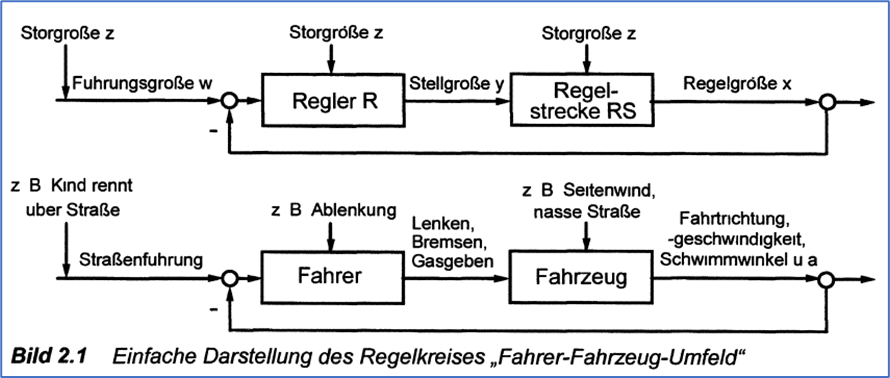
\includegraphics[width=\linewidth]{Bilder/FahrenRegelkreis.png}
	\caption{Einfache Darstellung des Regelkreises 	\glqq Fahrer-Fahrzeug-Umfeld\grqq{} \citep{Appel2002}} %TODO: Überall deutsche Anführungszeichen eingeben!!
	\label{fig:FahrenRegelkreis}
\end{figure}

Die \autoref{fig:FahrenRegelkreis} zeigt einen vereinfachten Regelkreis des Verhaltens zwischen den drei Komponenten (Fahrer-Fahrzeug-Umfeld). In dem Modell wurde die Ablenkung als ein Störgrößenbeispiel an den Fahrer und die nasse Straße als eine Störgröße ans Fahrzeug modelliert. Dieses Modell macht es leichter den Ablauf eines Unfalls zu verstehen und anschließend weitere Unfälle zu vermeiden. Durch eine Störung des Fahrers beziehungsweise des Fahrzeugs ändert sich der Ablauf einer Fahrt (oder eines Unfalls), da Störungen die Reaktionszeit sowie Reaktionsart der Fahrer stark beeinflussen. Diese sind im Fall eines Unfalls von großer Bedeutung. \\


%
\subsection{Zeitliche Phasen eines Unfalls}

Nach dem zeitlichen Unfallverlauf werden folgende Unfallphasen unterschieden:
\begin{itemize}
	\item Pre-Crash-Phase (Einlaufphase): 
	Die Einlaufphase beschreibt den Zeitraum vom Erkennen der kritischen Situation bis zum ersten Kontakt mit dem Hindernis beziehungsweise Unfallgegner.
	\item Crash (Kollisionsphase):
	Der Zeitraum vom ersten Kontakt zwischen den Unfallbeteiligten bis zur Lösung. Bei Mehrfachkollisionen werden mehrere Kollisionsphasen auftreten.
	\item Post-Crash-Phase (Folgephase):
	Die Folgephase ist der Zeitraum vom Lösen der Unfallbeteiligten bis zu ihrem Stillstand. Bei Mehrfachkollision treten auch mehrere Post-Crash-Phasen auf. 
	
\end{itemize}
Die Einlaufphase (Pre-Crash-Phase) ist maßgeblich vom Fahrer, der Straßenumgebung und der aktiven Sicherheit vom Fahrzeug abhängig (z.B. Bremsverhalten, Fahrzeugbeladung, gefährliche Kreuzungen, ...usw.).
 
Die Folgen der Kollisionsphase werden für die betroffenen Verkehrsteilnehmer maßgeblich durch die Maßnahmen der passiven Sicherheit (z.B. Lederkleidung beim Motorradfahrer) beeinflusst. Der Ablauf der Folgephase hängt stark von den verschiedensten Parametern beim Fahrzeug, beim Insassen und bei der Umgebung (z.B. Straßennässe) ab.\citep{Appel2002}\\


\subsubsection{Beispiel der Ablaufphasen einer Fahrsituation}

Die \autoref{fig:BeispielZeitlichePhasenEinesUnfalls} zeigt ein vereinfachtes Szenario einer kritischen Situation am Beispiel einer Kurve. Diese kritische Situation kann, muss aber nicht zwangsläufig zu einer Kollision führen. Zu einem bestimmten Zeitpunkt erkennt der Fahrer eine kritische Situation. Es ist zuerst unklar, ob es zu einem Unfall kommt. Nach dem Erkennen dieser Situation obliegt dem Fahrer die Entscheidung, welche Maßnahmen zu greifen sind, um eine Unfall-Situation zu vermeiden. Dabei wird der Fahrer auf bereits zurückliegende Erfahrungen zugreifen und eine zur Vermeidung dieser kritischen Situation geeignete Maßnahme ergreifen. Das Fahrzeug reagiert auf die Fahreraktionen, was zu '''Fahrer-Fahrzeug-Interaktion''' führt, die zu Unfällen führen.\citep{Appel2002}\\


\begin{figure}[H]
	\centering
	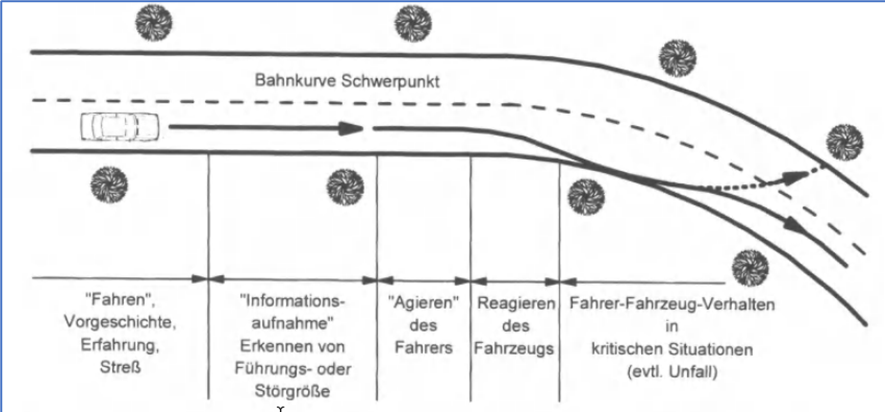
\includegraphics[width=\linewidth]{Bilder/BeispielZeitlichePhasenEinesUnfalls.png}
	\caption{Beispiel der zeitlichen Phasen einer kritischen Fahrsituation \citep{Appel2002}}
	\label{fig:BeispielZeitlichePhasenEinesUnfalls}
\end{figure}

%
%
%
%
%

\subsection{Statistische Zahlen über Motorradunfälle}
Das baden-württembergische Verkehrsministerium stellt ein Portal zur Verfügung, über das einzelne Verkehrsmessstellen abgefragt werden können. Die Messstationen wurden nach zwei Kriterien ausgewählt. Einerseits müssen Unfallschwerpunkte in unmittelbarer Nähe zu Messstationen sein, um zuverlässige Aussagen über Verkehr und Störstellen zu treffen.
Andererseits muss darauf geachtet werden, dass es keine Abzweigungen zwischen der Messstation und dem Unfallschwerpunkt gibt, da sonst das richtige Verkehrsaufkommen nicht erfasst werden kann.

Die \autoref{fig:GeschwUberschreitungPksMotorrad} stellt dar, wie oft die Geschwindigkeit von Motorradfahrer sowie von PKW-Fahrer an verschiedenen Stationen überschritten wurde. Aus der Grafik ist deutlich zu erkennen, dass an sechs der sieben Stationen das Geschwindigkeitslimit regelmäßig überschritten wird.
Die Motorradfahrer missachten die Geschwindigkeitsbegrenzung häufiger als die PKW-Fahrer. \citep{Maire2020}


\begin{figure}[H]
	\centering
	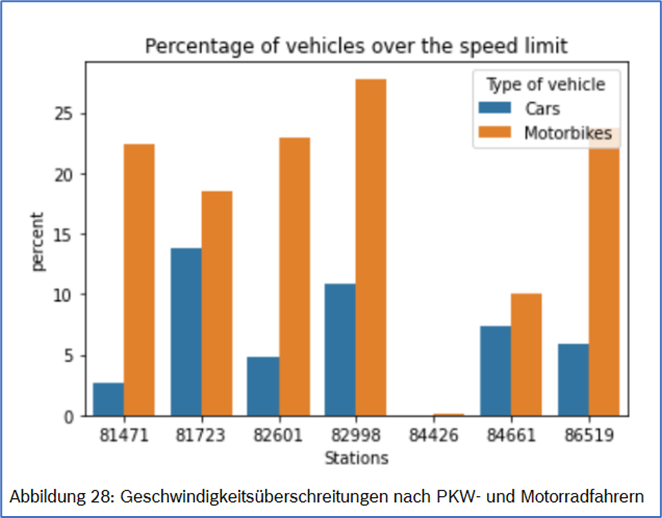
\includegraphics[width=\linewidth]{Bilder/GeschwUberschreitungPksMotorrad.png}
	\caption{Geschwindigkeitsüberschreitungen nach PKW- und Motorradfahrer an sieben Messstationen\citep{Maire2020}}
	\label{fig:GeschwUberschreitungPksMotorrad}
\end{figure}
Die GIDAS-Daten verfügen über die Ausgangsgeschwindigkeit des Motorradfahrers, was die Ermittlung des Einflusses dieser Geschwindigkeit auf die Unfallfolgen ermöglicht. In der \autoref{fig:SpeedSeverity} sind die Unfallschwere nach Motorradgeschwindigkeit als Histogramm dargestellt. Die Unfälle werden dabei nach Unfallschwere (leicht verletzt, schwer verletzt, tödlich verwundet) unterteilt. Die gestrichelten Linien repräsentieren die Mittelwerte der Histogramme.
Die Grafik zeigt, dass die Verletzungsschwere stark von der Geschwindigkeit abhängig ist. Bei einer $0$km/h gibt es keine tödliche Unfälle, wobei die Unfälle bei einer Geschwindigkeit von $100$ fast immer mit einer schweren Verletzung oder tödlichen Verkehrsteilnehmer enden. Die hohe Geschwindigkeit kommt immer mit hohen Kräfte zusammen, welche bei einem Unfall dem Fahrer bewirken. Im Fall eines Motorradfahrers ist das besonders wichtig zu betrachten, da diese Kräfte dem Fahrer direkt übertragen werden. \citep{Maire2020} %TODO: Einheit mit SIunit eingeben


\begin{figure}[H]
	\centering
	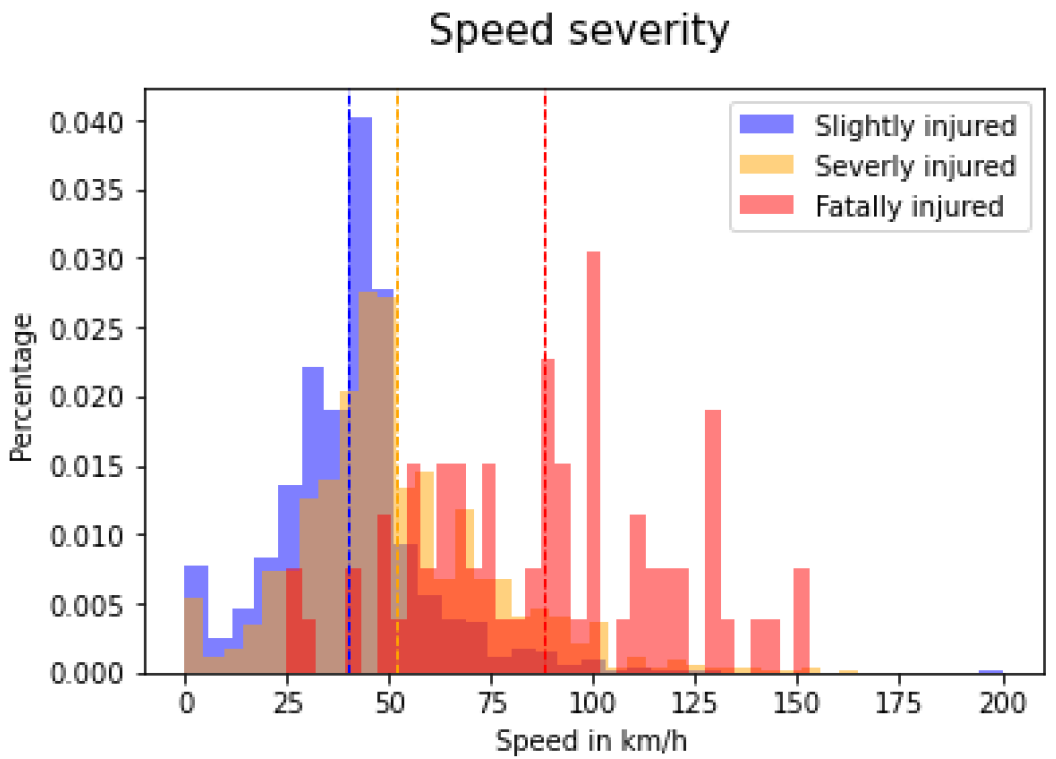
\includegraphics[width=\linewidth]{Bilder/SpeedSeverity.png}
	\caption{Unfallschwere über Geschwindigkeit aus der GAIDA-Datenbank\citep{Maire2020}}
	\label{fig:SpeedSeverity}
\end{figure}


%
%
%

\subsubsection{Statistische Zahlen aus mehreren Youtube-Videos} % TODO: neuer Überschrift!
%Meine Statistik aus Youtube-Videos\\

%Wie oft kommt welcher Unfall vor? (analog zu meiner BA)\\


Im Sinne der Verifizierung des angepassten Unfallerkennungsalgorithmus muss erstmals bekanntgegeben werden, welche Unfälle beziehungsweise Unfallarten am häufigsten vorkommen, damit diese tief betrachtet werden. Dazu wurden mehrere Videos von Motorradunfälle auf dem Plattform "'Youtube"' stichpunktartig angeschaut und die vorgestellten Unfälle statistisch analysiert. Es wurden insgesamt $32$ Unfallsituationen ausgewertet. In der Auswertung wurden die Unfallgegner und der Ablauf des Unfalls betrachtet. \citep{YTMotoCrashComp} \citep{YTCrazyDriverVsBiker} \citep{YTMotoCrashedAndMishaps} \citep{YTAnimalsVsBikers} \citep{YTMotoCrashesRoad}
\begin{figure}[H]
	\centering
	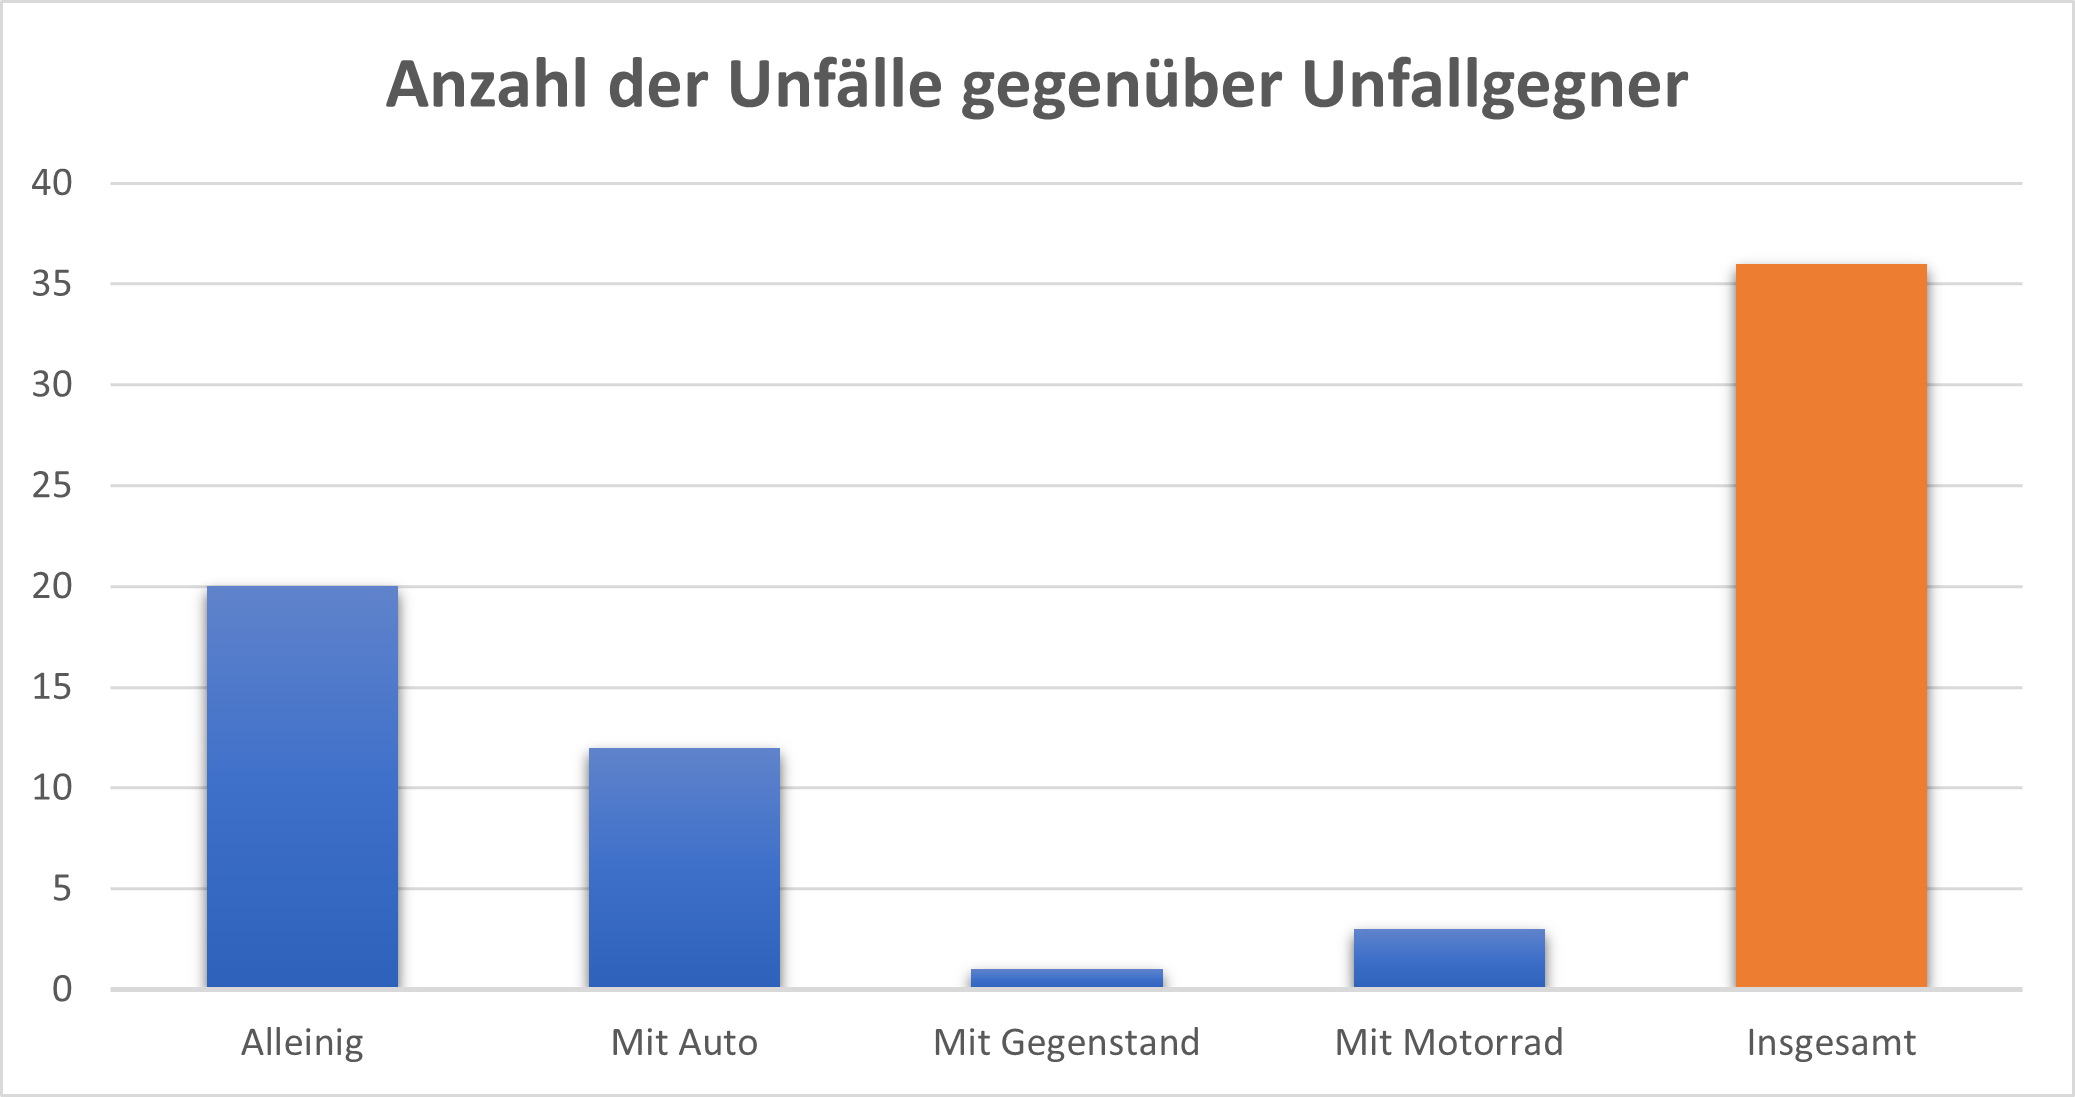
\includegraphics[width=\linewidth]{Bilder/youtube_Statistik_Unfallgegner.png}
	\caption{Anzahl der Unfälle gegenüber Unfallgegner}
	\label{fig:Youtube_Statistik_Unfallgegner}
\end{figure}
In der \autoref{fig:Youtube_Statistik_Unfallgegner} stellt die Grafik die Anzahl der Motorradunfälle gegenüber der Unfallgegner dar. Es wurde hier zwischen alleiniger Unfall, Unfall mit einem Gegner (Auto, Motorrad) oder Unfall wegen eines Gegenstands unterschieden. Diese Unterscheidung ist wegen der Verhaltensunterschied während eines Unfalls notwendig. Von insgesamt 36 Unfälle waren die alleinige Unfälle am meisten gefolgt von den Unfällen mit einem Auto. Die Unfälle mit einem anderen Motorrad oder wegen eines Hindernis sind am wenigsten. 
Unter alleinige Unfälle werden die zwei Szenarien (An einer Kurve rutschen und Kontrolle verlieren) am meisten aufgetreten, was sehr gut in der \autoref{fig:youtube_Statistik_AnzahlUnfallUrsachen} sichtbar sein kann. Das Szenario, in dem das Motorrad an ein Auto von hinten angestoßen hat, hatte die dritte Stelle besetzt. Die Hauptgründe der Unfällen mit einem Gegner waren vor Allem die hohe Geschwindigkeit und das schlechte Wetter (z.B. Nässe, Schnee), was zu Schwierigkeiten geführt hat, das Motorrad in kritischen Situationen zu kontrollieren.

Die \autoref{fig:youtube_Statistik_AktivPassivUnfall} zeigt den Anteil der aktiven sowie passiven Unfälle. Wenn das Motorrad angestoßen wird, wird von einem passiven Unfall gesprochen, da der Motorradfahrer keinen Einfluss darauf hat. Im Vergleich dazu könnte er bei einem aktiven Unfall das Ergebnis beeinflussen, in dem er langsamer fährt oder mehr Abstand mit den anderen Verkehrsteilnehmer hält.

\begin{figure}[H]
	\centering
	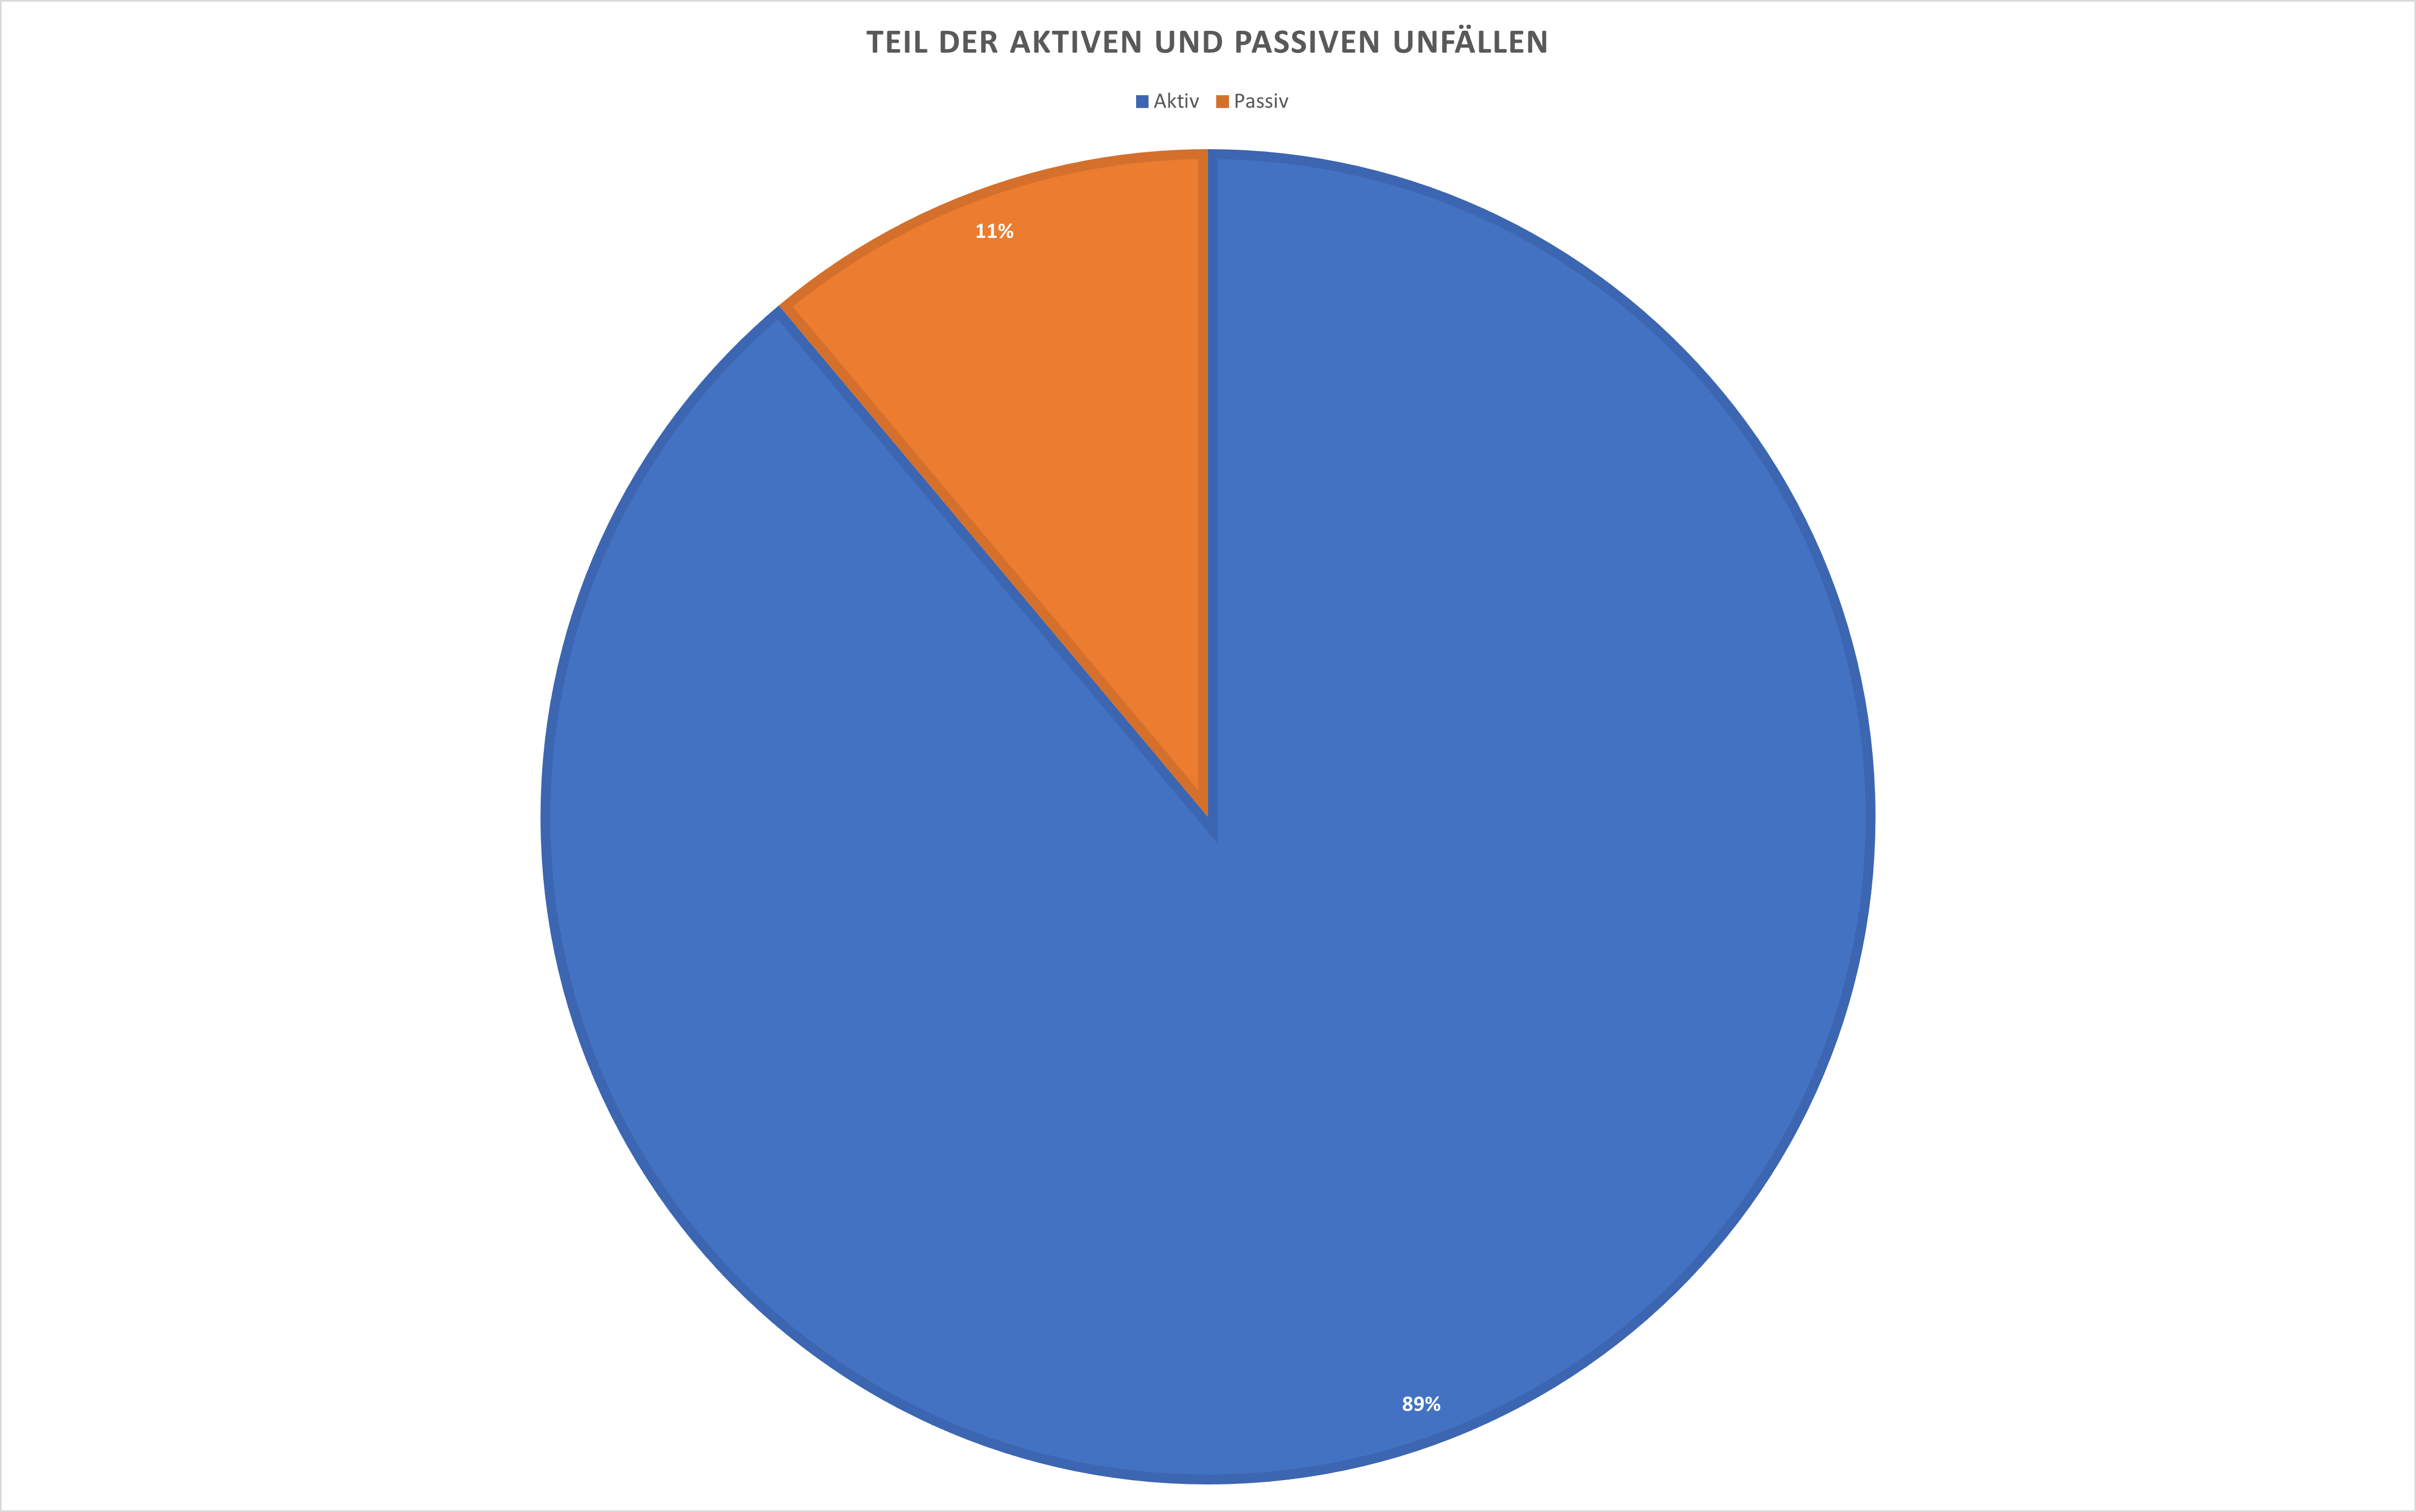
\includegraphics[width=\linewidth]{Bilder/youtube_Statistik_AktivPassivUnfall.png}
	\caption{Anteil der aktiven sowie passiven Unfälle}
	\label{fig:youtube_Statistik_AktivPassivUnfall}
\end{figure}

\begin{figure}[H]
	\centering
	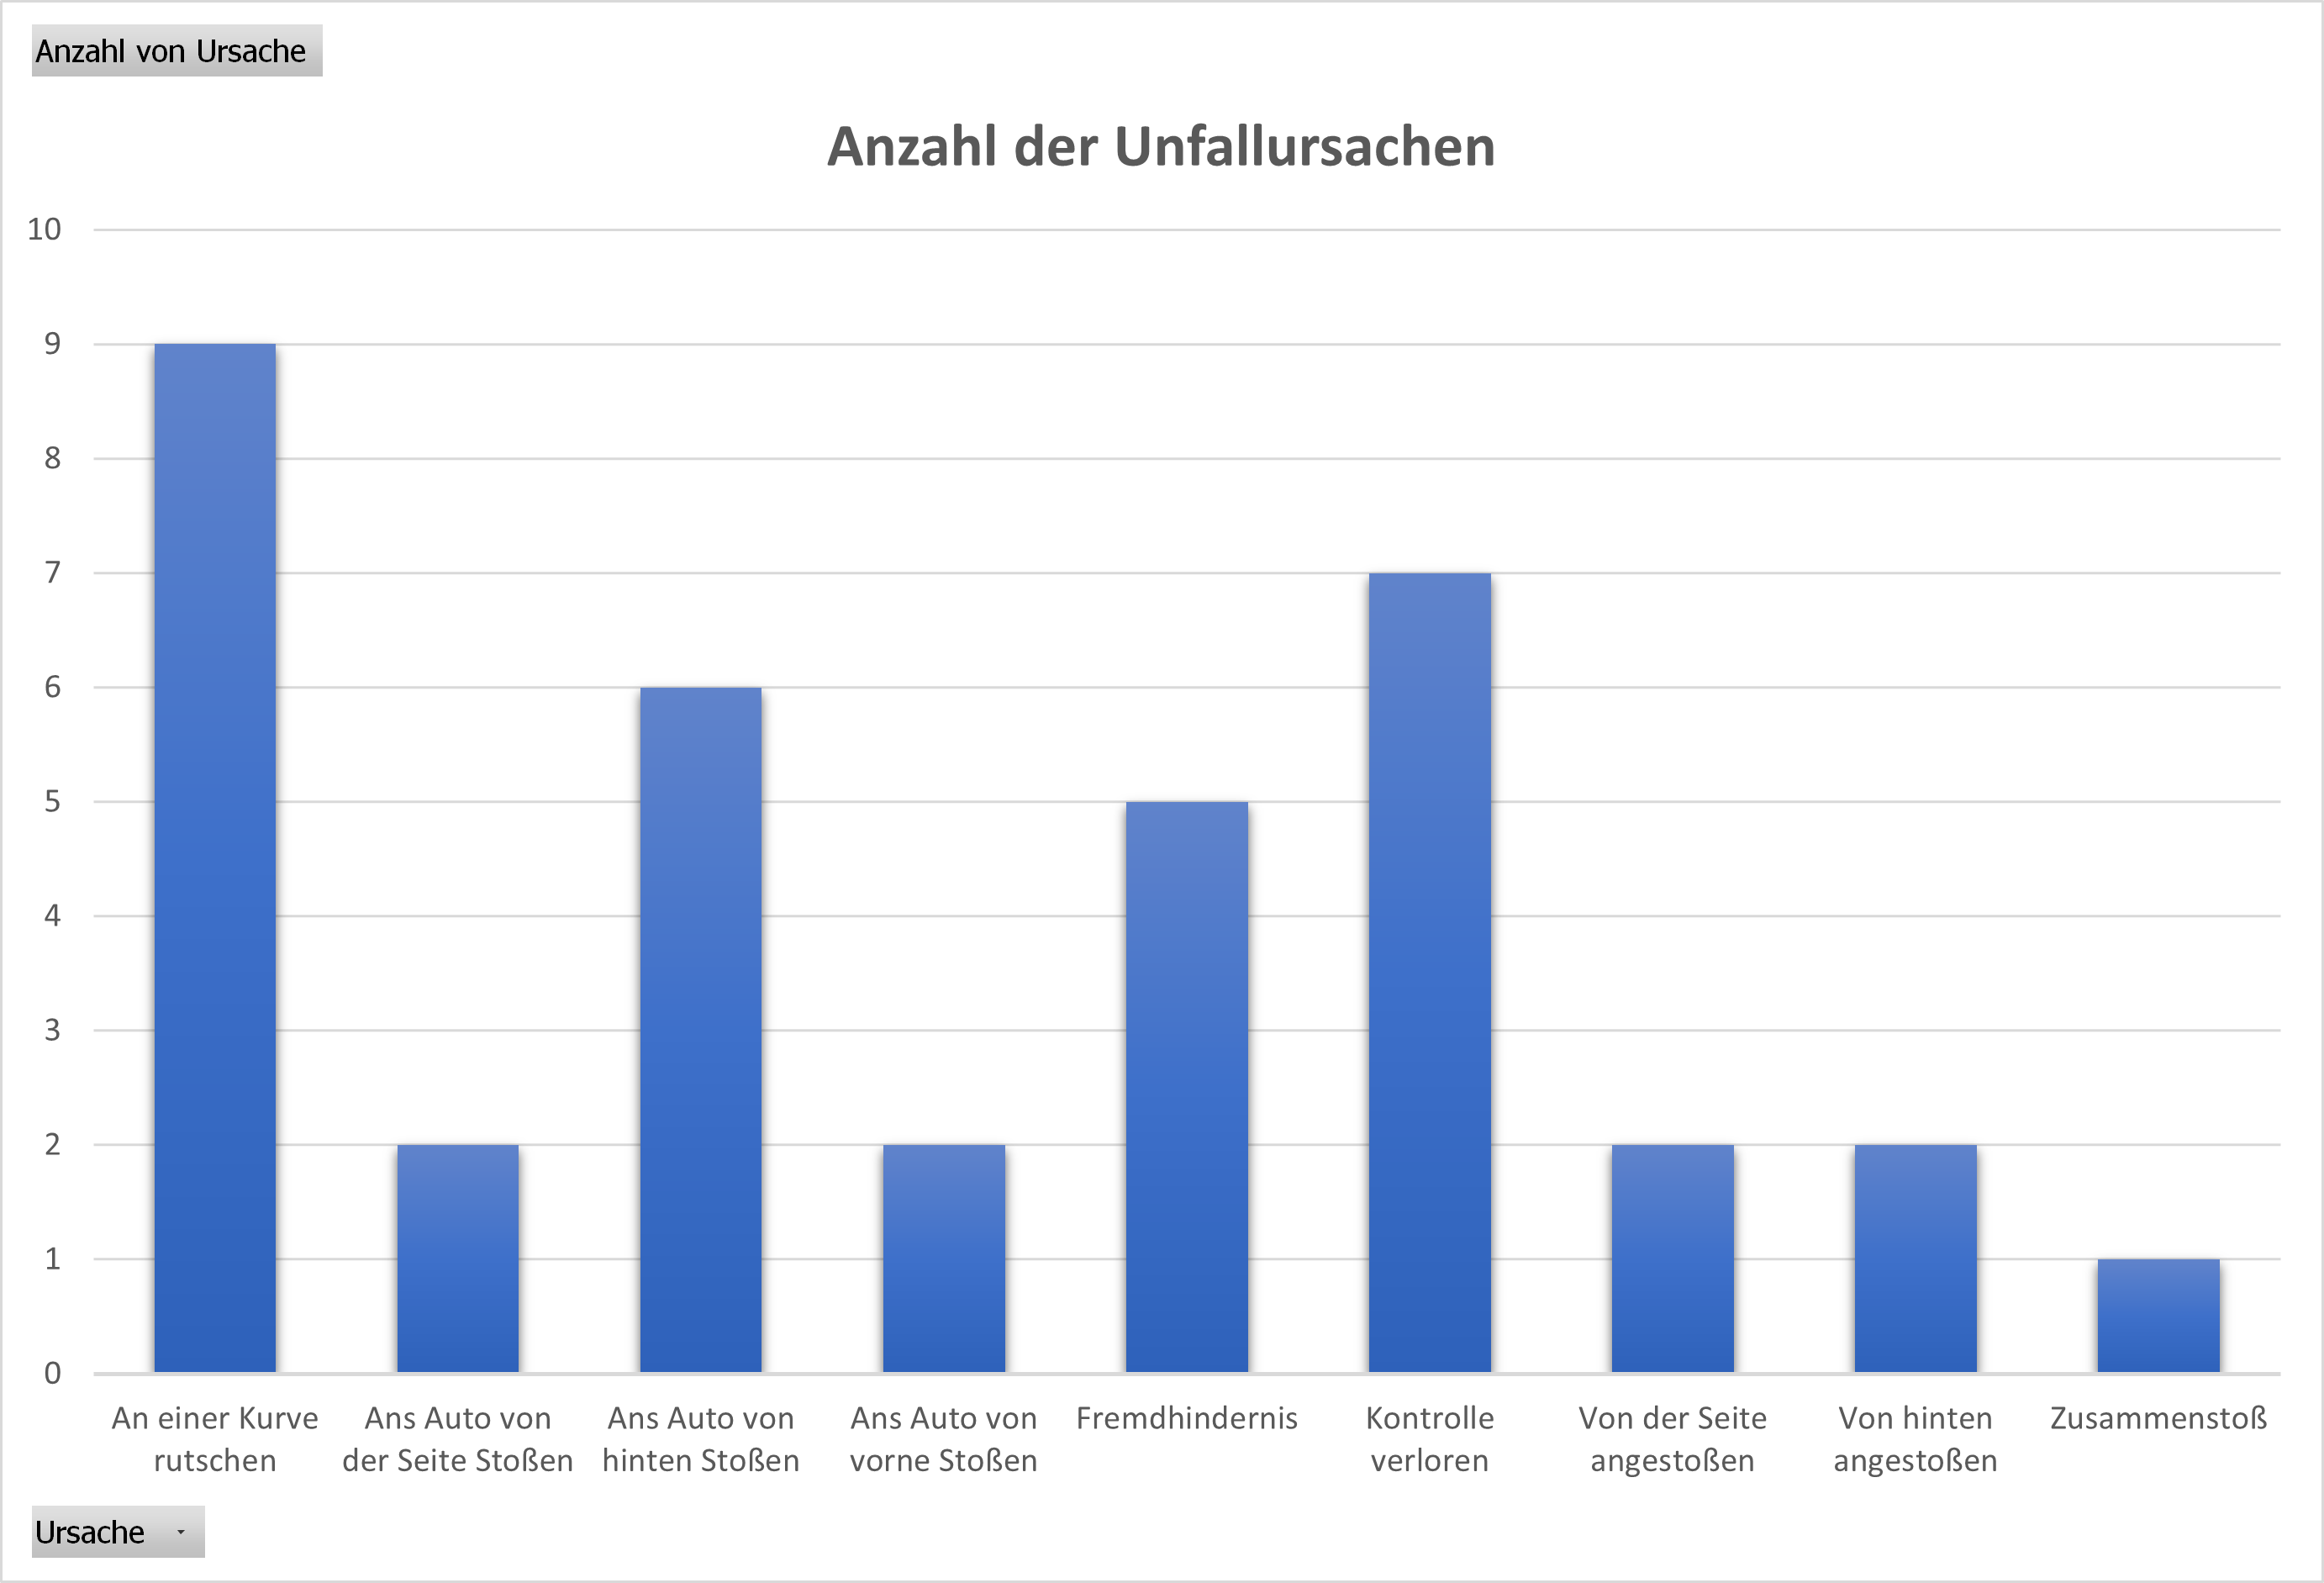
\includegraphics[width=0.9\linewidth]{Bilder/youtube_Statistik_AnzahlUnfallUrsachen.png}
	\caption{Anzahl der Unfälle über der Art der Ursache}
	\label{fig:youtube_Statistik_AnzahlUnfallUrsachen}
\end{figure}


Bilder aus den YT-Videos hinzufügen als Beispiele der Unfälle (vor Allem Alleiniger Unfall)


\subsection{Mechanik der Motorradfahrt} %Mechanik und Biomechanik des Unfalls
- Kinematik und Verletzungsbilder\\
- Zweiradfahrer (Bilder)

\subsubsection{Kurvenfahrt} 

Der Fahrer bestrebt während der Fahrt immer das Gleichgewicht zu halten, damit er und das Motorrad nicht umkippt. Bei einer Geradeausfahrt und ab einer Geschwindigkeit von $25$ km/h stabilisieren die Kreiselkräfte der Räder die Maschine. Bei einer Geschwindigkeit unter $25$ km/h reichen die Kreiselkräfte nicht mehr aus, um das Gleichgewicht zu gewährleisten und der Fahrer muss mit kleinen Lenkausschlägen von bis zwei Grad nach links und rechts die Gleichgewichtslage halten.\\
Befährt ein Motorradfahrer eine Kurve, tritt im Vergleich zu einer Geradeausfahrt eine Instabilität im Gleichgewicht auf und versucht der Fahrer die Maschine wieder zum Gleichgewicht zu bringen. Während der gesamten Kurvenfahrt kann der Fahrer den Verlauf der Fahrlinie sowohl durch positives oder negatives Beschleunigen als auch durch die Veränderung des Lenkwinkels beeinflussen. \citep{Haedrich2012} 


\subsubsection{Wirkende Kräfte am Fahrzeugschwerpunkt}

Beim Einleiten einer Kurvenfahrt mit konstantem Bahnradius wirkt eine konstante Querbeschleunigung ($a_q$) auf die Einheit ''Fahrer-Maschine''. Diese Querbeschleunigung bewirkt eine Seitenkraft im Gesamtschwerpunkt der Einheit ''Fahrer-Maschine''. %und wird wie folgt berechnet:
%\begin{align}
%	\centering
%	a_q = \frac{v^2}{R} = \frac{1}{D}
%	\label{gl:Querbeschleunigung}
%\end{align}

Die \autoref{fig:VereinfachteDarstellungDerKraefteBeiStationaererKurvenfahrt} zeigt die wirkenden Kräfte und die daraus resultierenden Momente während der stationären Kurvenfahrt an einem vereinfachten Modell. Die Gewichtskraft $F_G = m_g \cdot g$ sowie die Fliehkraft beziehungsweise Zentrifugalkraft $F_a = m_g \cdot a_q$ sind in der Abbildung ersichtlich. Die Fliehkraft versucht das Motorrad nach Außen zum Kippen zu bringen, deswegen wird das Fahrzeug die Kurve unter Schräglage durchzufahren. Dadurch verschiebt sich der Schwerpunkt der Einheit zur Kurvenseite und wird ein Moment der Gewichtskraft um den Reifenaufstandspunkt resultiert, welches dem Moment der Fliehkraft entgegen wirkt und wieder ein Gleichgewicht sichert.

Der Schrägwinkel ($\lambda$) der Einheit lässt sich wie folgt berechnet:


\begin{align*}
	\centering
	\tan(\lambda)  =  \frac{F_a}{F_G}
\end{align*}
\begin{align}
	\centering
	\lambda  =  \arctan \left(\frac{F_a}{F_G}\right)
	\label{gl:Schraegwinkel}
\end{align}


\begin{figure}[H]
	\centering
	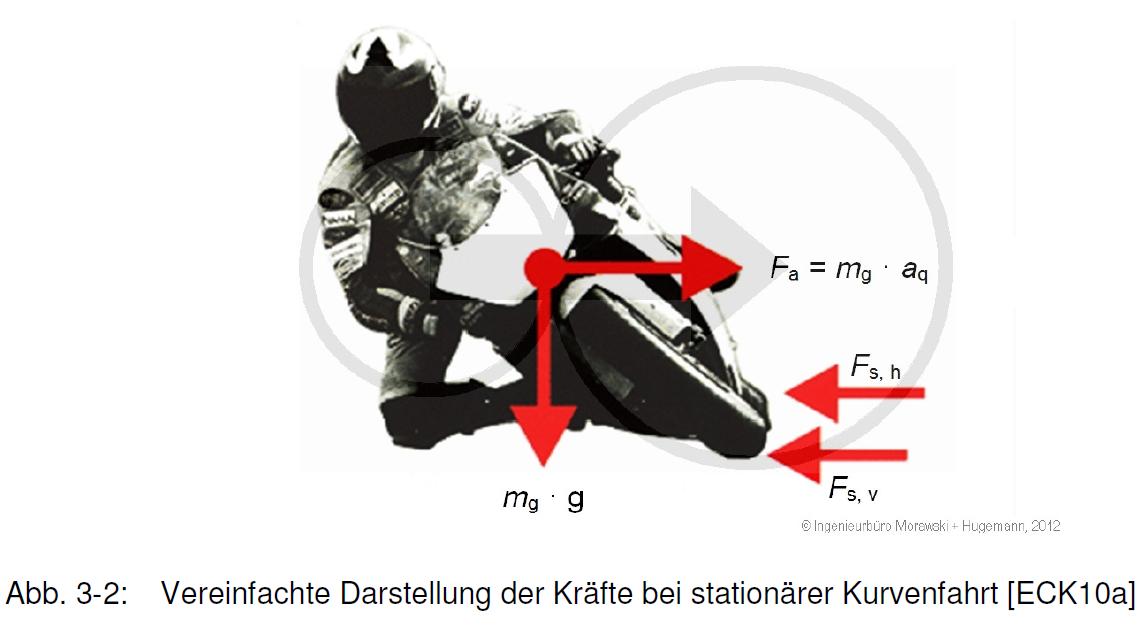
\includegraphics[width=\linewidth]{Bilder/VereinfachteDarstellungDerKraefteBeiStationaererKurvenfahrt.png}
	\caption{Vereinfachte Darstellung der Kräfte bei stationärer Kurvenfahrt)}
	\label{fig:VereinfachteDarstellungDerKraefteBeiStationaererKurvenfahrt}
\end{figure}


\textbf{Kurventechniken:}\\
Die bisherigen Überlegungen und Berechnungen beziehen sich jeweils auf den Fall, dass der Fahrer während der Kurvenfahrt in einer Flucht mit der Maschinenachse bleibt. Tatsächlich gibt es jedoch verschiedene Techniken, eine Kurve durchzufahren, vgl. (\autoref{fig:VerschiedeneKurventechnikenbeigleicherGeschwindigkeit}).
\begin{figure}[H]
	\centering
	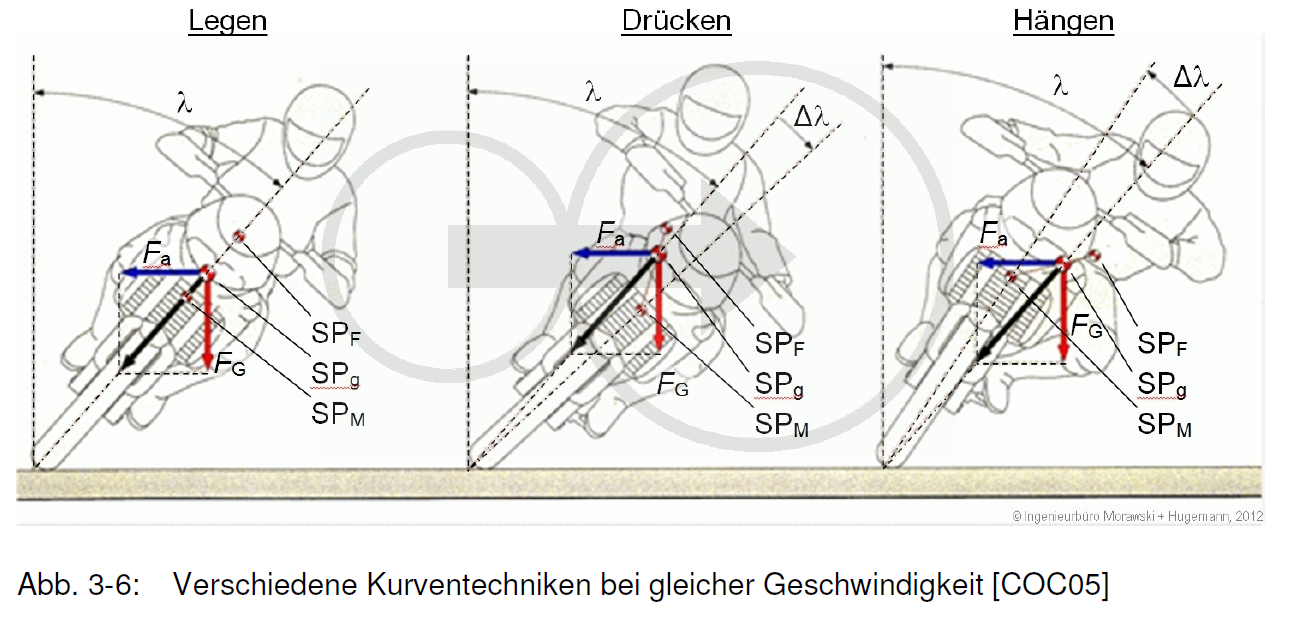
\includegraphics[width=\linewidth]{Bilder/VerschiedeneKurventechnikenbeigleicherGeschwindigkeit.png}
	\caption{Verschiedene Techniken bei Kurvenfahrt mit gleicher Geschwindigkeit}
	\label{fig:VerschiedeneKurventechnikenbeigleicherGeschwindigkeit}
\end{figure}

Der Fahrstil „Drücken“ hat im Vergleich zum Fahrstil „Legen“ keinen Vorteil im Zusammenhang des Grips auf der Straße. Es ist durchaus vorstellbar, dass mit zunehmender Schräglage die Reifenaufstandsfläche (beziehungsweise Reifenlatsch) abnimmt.

Fahrer von Renn- und Supersport-Maschinen bedienen sich der Tatsache des sich verändernden Reifenlatsches und „Hängen“ sich während der Kurvenfahrt von der Maschine. In diesem Fall liegt der Schwerpunkt des Fahrers SPF unterhalb des Schwerpunktes der Maschine SPM, so dass das Motorrad die Kurve mit deutlich geringerer Schräglage durchfahren kann, als beim „Legen“, (\autoref{fig:VerschiedeneKurventechnikenbeigleicherGeschwindigkeit}). Gegenüber der anderen zwei Schräglagen kann durch das ''Hängen'' mit gleichen Schrägwinkel höhere Seitenkräfte übertragen werden, da hier die Radaufstandsfläche größer ist.


%
%
%
%
\section{Technische Grundlagen} \label{Technik}



\subsection{Sensoren und Signale der Smartphones}

%
%
%
%
%
Die meisten Smartphones haben einen Beschleunigungsmesser, und viele enthalten jetzt ein Gyroskop. Je nach Gerät können die softwarebasierten Sensoren ihre Daten entweder vom Beschleunigungs- und Magnetometer oder vom Gyroskop beziehen. Diese Sensoren sind nützlich zum Überwachen von Gerätebewegungen wie Neigung, Schütteln, Drehung oder Schwingen. Die Gerätsbewegung spiegelt normalerweise die direkte Benutzereingabe wider, kann aber auch die physische Umgebung widerspiegeln, in der sich das Gerät befindet (z.B. Das Smartphone bewegt sich mit der Person, die es am Körper hat und sich selbst bewegt).\citep{DevelopersMotionSen}



%
%
%
%


\subsubsection{Beschleunigungssensoren}
- Beispielsignal\\

Der Beschleunigungssensor ist ein elektromechanisches Gerät, das die Beschleunigungskraft misst, die durch Bewegung, Schwerkraft oder Vibration verursacht wird. Mathematisch gesehen ist die Beschleunigung ein Maß für die zeitliche Geschwindigkeitsänderung.
Der Beschleunigungssensor im Smartphone misst die lineare Beschleunigung des Geräts. In der Ruheposition stellt die Figur die auf das Gerät wirkende Schwerkraft dar und misst gleichzeitig auch die Beschleunigung auf der X- und Y-Achse, die Null sein wird.
Die meisten Smartphones verwenden heutzutage Beschleunigungssensoren, um die Bildschirmanzeige abhängig von der Position auszurichten, in der das Gerät gehalten wird. Mit den eingebauten Beschleunigungssensoren können Benutzer unter Anderem ein besseres Anzeigeerlebnis erzielen. \citep{Sharma2020}

Der Beschleunigungssensor im mobilen Gerät liefert die XYZ-Koordinatenwerte, die zum Messen der Position und der Beschleunigung des Geräts verwendet werden. Die XYZ-Koordinate stellt die Richtung und Position des Geräts dar, an dem eine Beschleunigung aufgetreten ist. Die Drehrichtung und -position werden mit Gyroskopsensoren gemessen. Die vom Gerät bereitgestellten Beschleunigungsmesserwerte enthalten normalerweise auch die Schwerkraft. Das Signal des Beschleunigungssensor wird in die Tief-/Hochpassfilter geleitet, um das Ergebnis basierend auf der verwendeten Anwendung zu verfeinern. \citep{Sathish2021}
\begin{itemize}
	\item Wird das Gerät auf die linke Seite geschoben (bewegt sich also nach rechts), ist der x-Beschleunigungswert positiv.
	\item Wenn das Gerät auf seinen Boden gedrückt wird, ist der y-Beschleunigungswert positiv.
	\item Wenn das Gerät mit einer Beschleunigung von A m/s2 in den Himmel geschoben wurde, ist der Wert der z-Beschleunigung gleich A + 9,81, da die Schwerkraft (9,81 m/s2) mitberechnet wird.
	%TODO: Beispielsignale hinzufügen
\end{itemize}
Im Allgemeinen ist der Beschleunigungssensor ein guter Sensor, wenn die Bewegung des Geräts überwacht werden soll. \citep{DevelopersMotionSen}

%
%
%
%
\subsubsection{Gyroskop}
- Beispielsignal\\

Gyroskop ist ein Gerät, das ein sich schnell drehendes Rad oder einen umlaufenden Lichtstrahl enthält. Gyroskop wird verwendet, um die Abweichung eines Objekts von seiner gewünschten Ausrichtung zu erkennen. Gyroskope werden zur automatischen Lenkung und zur Korrektur der Dreh- und Nickbewegung in Marschflugkörpern und ballistischen Flugkörpern verwendet.\citep{RogersGyro}
Der Gyroskopsensor im MEMS ist winzig (zwischen 1 und 100 Mikrometer). Wenn der Gyro gedreht wird, wird eine kleine Resonanzmasse bei einer Winkelgeschwindigkeitsänderung verschoben. Diese Bewegung wird in elektrische Signale mit sehr geringem Strom umgewandelt, die verstärkt und von einem Host-Mikrocontroller gelesen werden können.\citep{sparkfunGyro}


%\subsubsection{Achsenrichtung im Smartphon}
%- Unterschied zwischen Android und IOS
%
%Im Allgemeinen verwendet das Sensor-Framework ein standardmäßiges 3- Achsen-Koordinatensystem, um Datenwerte auszudrücken. Bei den meisten Sensoren wird das Koordinatensystem relativ zum Bildschirm des Geräts definiert, wenn das Gerät in seiner Standardausrichtung gehalten wird.
%Der wichtigste Punkt, den es bei diesem Koordinatensystem zu verstehen gilt, ist, dass die Achsen nicht vertauscht werden, wenn sich die Bildschirmausrichtung des Geräts ändert. \citep{DevSensorOver}
%
%Die \autoref{fig:Achsenrichtung_Android} zeigt die Referenz-Achsenrichtung in einem typischen Android-Smartphone. Das Koordinatensystem ist zum Bildschirm des Geräts definiert.
%
%
%\begin{figure}[H]
%	\centering
%	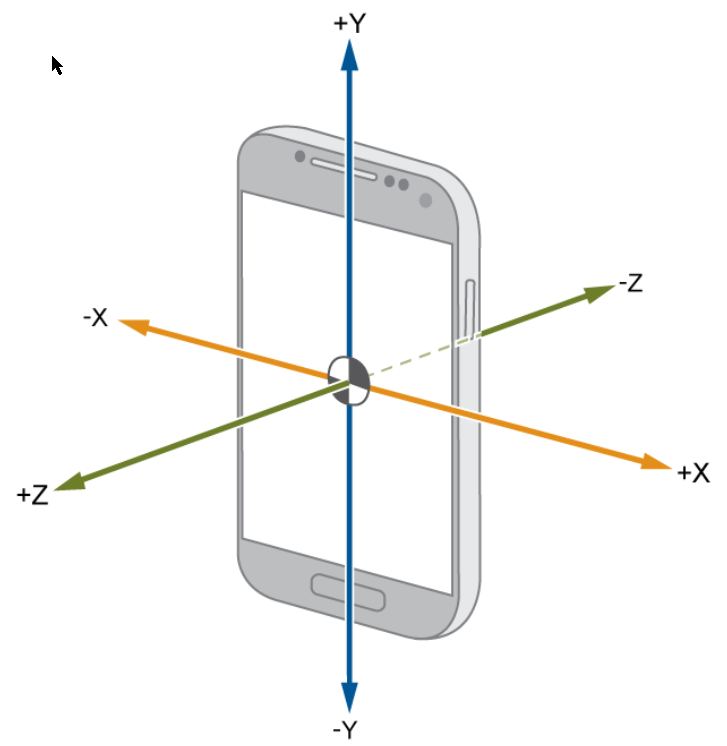
\includegraphics[width=0.5\linewidth]{Bilder/Achsenrichtung_Android.png}
%	\caption{Achsenrichtung in einem Android-Smartphone\citep{Mathworks}}
%	\label{fig:Achsenrichtung_Android}
%\end{figure}

\subsubsection{Global Positioning System (GPS)}
%- Aufbau kurz erläutern\\
%- Geschwindigkeit mit GPS messen\\
%- Beispielsignal\\

GPS besteht aus drei Teilen: Satelliten, Bodenstationen und Empfängern. Die Position der Satelliten ist jederzeit bekannt. Die Bodenstationen verwenden Radar, um sicherzustellen, dass die Satelliten sich tatsächlich dort sind, wo sie sich befinden sollen.
Ein Empfänger in dem Smartphone oder im Auto wartet ständig auf ein Signal von diesen Satelliten und findet heraus, wie weit er von einigen von diesen Satelliten entfernt ist. Sobald die Entfernung zwischen einem Empfänger und vier oder mehr Satelliten berechnet wurde, ist genau bekannt, wo der Empfänger sich befindet. Der Basis-GPS-Dienst bietet Benutzern eine Genauigkeit von etwa 7,0 Metern, 95\% der Zeit. GPS-Empfänger zeigen die Geschwindigkeit an und berechnen die Geschwindigkeit mithilfe von Algorithmen im Kalman-Filter.\citep{Nasa2019}\citep{FAAGPS}\citep{YeazelGPS}

%
%
%
%

\subsection{Integrierte Aktivitätserkennung}

- Es gibt vom Google eine integrierte Aktivitätserkennung.\\

- Beispielsignal\\

- Das Ergebnis ist die Wahrscheinlichkeit pro Aktivität.\\

- Eine Darstellung hinzufügen. In der Abb. sind zwei Grafiken: 1. Acc-Signal bei verschiedenen Aktivitäten. 2. Eine Aktivitätsklassifizierung. mit einer Phasenunterscheidung!

\subsection{Matlab/Simulink}
%- warum Matlab/Simulink und nicht direkt C oder LabView\\

Matlab ist eine Hochleistungssprache für technisches Rechnen. Matlab integriert Berechnung, Visualisierung und Programmierung in einer benutzerfreundlichen Umgebung, in der Probleme und Lösungen in einer vertrauten mathematischen Notation ausgedrückt werden.

Simulink ist ein grafisches Softwarepaket zur Modellierung, Simulation und Analyse dynamischer Systeme und basiert auf Matlab. 
Die Software hat sich in den letzten Jahren zum weitesten verbreiteten Softwarepaket in Wissenschaft und Industrie entwickelt.
Simulink unterstützt lineare und nichtlineare Systeme, die in kontinuierlicher Zeit, gesampelter Zeit oder einer Mischung aus beiden modelliert sind. Für die Modellierung bietet Simulink eine grafische Benutzeroberfläche (GUI) zum Erstellen von Modellen als Blockdiagramme. Mit dieser Schnittstelle können die gewünschten dynamischen Systeme einfach aufgebaut werden. Mithilfe von Scopes und anderen Anzeigeblöcken können die Simulationsergebnisse während der Simulation analysiert werden. Die Simulationsergebnisse können zur Nachbearbeitung und Visualisierung in den MATLAB-Arbeitsbereich gestellt werden. \citep{Iov2004}\citep{Karris2008}\\



\subsubsection{Simulink und LabVIEW} 
LabVIEW ist eine von "National Instruments'' entwickelte Software. Sie wird häufig von Ingenieuren, Wissenschaftlern und Studenten für die Datenerfassung, Instrumentensteuerung und industrielle Automatisierung verwendet. Die LabVIEW-Umgebung besteht aus zwei Hauptkomponenten: Frontpanel (FP) und Blockdiagramm (BD). Ein FP stellt die grafische Benutzeroberfläche bereit, während ein BD die Bausteine eines Systems enthält und einem Flussdiagramm ähnelt. LabVIEW-Systeme werden als virtuelle Instrumente (VIs) bezeichnet und ihr FP erscheint als Instrumententafel, die aus verschiedenen Bedienelementen und Anzeigen besteht.

Ähnlich wie LabVIEW bietet Simulink einen blockbasierten Programmieransatz für die Simulation, den Entwurf und die Analyse dynamischer Systeme. Es bietet eine interaktive grafische Umgebung zusammen mit einer Reihe von Bibliotheken zum Entwerfen und Simulieren von Systemen, einschließlich DSP-Systemen. Simulink-Blöcke werden als Modelle bezeichnet, und im Gegensatz zu LabVIEW werden die Codeimplementierung und Eingabe-/Ausgabeeinheiten in Simulink nicht explizit unterschieden. Simulink ist in MATLAB integriert und kann daher auf die Funktionen und Tools zugreifen, die in der MATLAB-Umgebung verfügbar sind. \citep{Kehtarnavaz2006} \citep{Cansalar2015}\\

%Quelle: https://stackoverflow.com/questions/17185249/extensive-comparison-between-simulink-and-labview

Wenn komplexe Simulationen ausgeführt werden sollen oder komplexe Simulationsmodelle von Steuerungen oder Anlagen zu erstellen/debuggen sind, wird Simulink verwendet, da LabVIEW keine effizienten Codegeneratoren für die dynamische Simulation hat.
Simulink konzentriert sich hauptsächlich auf Simulation und Modellierung, was bei LabVIEW sicherlich nicht der Fall ist.

Der implemntierte Algorithmus enthält einen verbreiteten und komplexen Entscheidungsbaum, welcher sich mit Simulink sowohl übersichtlicher als auch einfacher darstellen lässt als mit LabVIEW.



\subsubsection{App-Entwicklung}
Die Entwicklung mobiler Apps ist der Prozess zur Erstellung von Software für Smartphones und digitale Assistenten. Die Software kann auf dem Gerät vorinstalliert oder aus einem mobilen App Store heruntergeladen werden. Eine der bekannten Sprachen in der App-Entwicklung ist C.
C ist eine leistungsstarke Programmiersprache, mit der Anwendungen in mehreren Bereichen erstellt werden können, von einfachen Taschenrechnern und Apps bis hin zu Videospielen. Sie ist eine Sprache auf niedriger Ebene, dies bietet Geschwindigkeit und eine weitaus bessere Möglichkeit zur Speicherverwaltung.

Für die Generierung eines C-Codes aus Simulink-Modellen wird der in Matlab/Simulink integrierte C/C++-Coder verwendet. *******Quelle******* %TODO: Quelle

\subsubsection{C/C++-Coder}
Der C/C++-Code-Generator wird für Rapid Prototyping, Hardware-in-the-Loop-Tests, Simulationsbeschleunigung oder einfach als ausführbare Datei zur Ausführung außerhalb von MATLAB und Simulink verwendet.
Diese Codegenerierung ist der Prozess der Generierung von Low-Level-Code direkt aus einer High-Level-Programmiersprache oder Modellierungsumgebung.

Der C/C++-Coder ist ein weiterer Vorteil von Simulink gegenüber LabVIEW und hierfür ist Simulink die richtige Entscheidung für die Implementierung der Software beziehungsweise des Unfallerkennungsalgorithmus'.






\section{Mathematische Grundlagen}

In dieser Arbeit wird eine FFT eingesetzt, für welche das folgende Hintergrundwissen zum Verständnis benötigt wird.
\subsection{Fast Fourier Transform (FFT)} \label{abs:FFT}

Die „Fast Fourier Transform“ ist ein wichtiges Messverfahren und wurde erstmals von Cooley und Tukey 1965 diskutiert, obwohl Gauß den kritischen Faktorisierungsschritt bereits 1805 beschrieben hatte. Dieses Verfahren wandelt ein Signal in einzelne Spektralkomponenten um und liefert dadurch Frequenzinformationen über das Signal. FFT wird zur Fehleranalyse, Qualitätskontrolle und Zustandsüberwachung von Maschinen oder Anlagen eingesetzt. Dieser Abschnitt erläutert die Funktionsweise einer FFT, die relevanten Parameter und deren Auswirkungen auf das Messergebnis.
Die FFT ist ein optimierter Algorithmus zur Umsetzung der „Diskrete Fourier Transformation“ (DFT). Ein Signal wird über einen Zeitraum abgetastet und in seine Frequenzkomponenten zerlegt. Diese Komponenten sind einzelne sinusförmige Schwingungen mit unterschiedlichen Frequenzen, jede mit ihrer eigenen Amplitude und Phase. Diese Transformation ist an einem Beispiel in der \autoref{fig:FFTBeispiel} dargestellt.\\
%Über den gemessenen Zeitraum enthält das Signal drei unterschiedliche dominante Frequenzen.\\
Das Diagramm zeigt ein kompliziertes Signal im Zeitbereich, das aus der Summe der drei periodischen Grundsignalen mit unterschiedlichen Frequenzen entsteht. Im Frequenzbereich sind u.A. die einzelne Frequenzen der Grundsignalen dargestellt. Dadurch lässt sich eine FFT-Transformation zwischen dem Zeit- sowie Frequenzbereich grafisch darstellbar.

\begin{figure}[H]
	\centering
	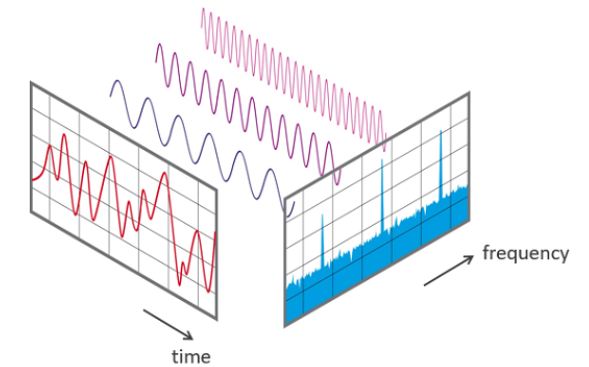
\includegraphics[width=0.5\linewidth]{Bilder/FFTBeispiel.png}
	\caption{Beispiel von einer FFT (Zeitbereich und Frequenzbereich)\citep{NTIAudioFFT}}
	\label{fig:FFTBeispiel}
\end{figure}

\subsubsection{Schritt für Schritt}
Im ersten Schritt wird ein Ausschnitt des Signals abgetastet und zur weiteren Verarbeitung im Speicher abgelegt. Zwei Parameter sind hier relevant:
\begin{enumerate}
	\item Die Abtastrate beziehungsweise Abtastfrequenz $f_s$ des Messsystems (z.B. $48$ kHz). Dies ist die durchschnittliche Anzahl von Abtastungen, die in einer Sekunde erhalten werden (Abtastungen pro Sekunde)
	\item Die Blocklänge $B_L$ ist die ausgewählte Anzahl von Proben (Samples). Dies ist immer eine ganzzahlige Potenz zur Basis 2 (z.B. $2^{10}=1024$ Samples)
\end{enumerate}
Aus den beiden Grundparametern $f_s$ und $B_L$ können weitere Parameter der Messung bestimmt werden. \\
\textbf{Bandbreite:}  $f_n$ (= Nyquist-Frequenz). Dieser Wert gibt die theoretische maximale Frequenz an, die durch die FFT bestimmt werden kann.
\begin{align}
	\centering
	f_n = \frac{f_s}{2}
	\label{gl:Nyquist-Frequenz}
\end{align}
Beispielsweise können bei einer Abtastrate von $100$ Hz Frequenzanteile bis $50$ Hz bestimmt werden.\\
\textbf{Messdauer:} $D$ ergibt sich aus der Abtastrate $f_s$ und der Blocklänge $B_L$ wie folgt:

\begin{align}
	\centering
	D = \frac{B_L}{f_s}
	\label{gl:Messdauer}
\end{align}
\textbf{Frequenzauflösung:} $d_f$ gibt den Frequenzabstand zwischen zwei Messergebnissen an.
\begin{align}
	\centering
	d_f = \frac{f_s}{B_L} = \frac{1}{D}
	\label{gl:Frequenzaufloesung}
\end{align}
In der Praxis ist die Abtastfrequenz $f_s$ meist eine vom System vorgegebene Größe. Durch die Auswahl der Blocklänge $B_L$ kann jedoch die Messdauer $D$ und Frequenzauflösung $d_f$ definiert werden. Es gilt:\\
\begin{itemize}
	\item Eine kleine Blocklänge $B_L$ führt zu schnellen Messwiederholungen mit grober Frequenzauflösung.
	\item Eine große Blocklänge $B_L$ führt zu langsameren Messwiederholungen mit feiner Frequenzauflösung.
\end{itemize}
\subsubsection{Spiegelfrequenzen}
Wird die Nyquist-Frequenz (\autoref{gl:Nyquist-Frequenz}) überschritten, wird das Signal an dieser gedachten Grenze reflektiert und fällt wieder in das Nutzfrequenzband zurück. Diesen unerwünschten Spiegelfrequenzen wird vor der Abtastung mit einem analogen Tiefpassfilter (Anti-Aliasing-Filter) entgegengewirkt. Der Filter sorgt dafür, dass Frequenzen oberhalb der Nyquist-Frequenz unterdrückt werden. \citep{NTIAudioFFT}\citep{WeissteinFFT}






%
%
%
%
%
%
%



\section{Agile Softwareentwicklung}\label{abs:MethodenderSoftwareentwicklung}
Das Ziel der agilen Softwareentwicklung ist die kontinuierliche Bereitstellung funktionsfähiger Software, die in schnellen Iterationen erstellt wird. 
Die agile Softwareentwicklung ermöglicht eine kontinuierliche Bereitstellung funktionsfähiger Software, die in schnellen Iterationen erstellt wird. Bei einer agilen Softwareentwicklung werden die Entwicklungsphasen in mehreren Sprinten geteilt. Die Länge einer Sprint wird am Anfang festgestellt. Nach jedem Sprint wird das Ergebnis ausgewertet. Dieses wird ggf. für die Anpassung des Entwicklungsvorgehens im nachfolgenden Sprinte benutzt\citep{Brunskill2019}.
Die Entwicklung des Unfallerkennungsalgorithmus' sowie das Pocket-Mode wird mittels der agilen Methode erfolgt. 


%
%
%
%
%
%
%
\section{Unfallerkennungsalgorithmus} \label{abs:Unfallerkennungsalgorithmus}
% TODO: besser formulieren
% TODO: Eine Skizze des Ablaufs der Unfallerkennungsschritte (Unfallerkennung -> Agent -> Rettungsdienst ...usw.)
%
%
%
%

In diesem Teil wird der Unfallerkennungsalgorithmus erläutert und näher betrachtet. Der Algorithmus ist sowohl für Fahrräder als auch für Motorräder entwickelt und bearbeitet die Signale der Beschleunigungssensor sowie Gyroskope im Smartphone und die über Gps gemessene Geschwindigkeit. In dem Unfallerkennungsalgorithmus werden drei Hauptkriterien (CollisionHit, GroundHit und TipOver) berücksichtigt.

Die Modellierung der Merkmale GroundHit und Collision erfordert weitere unabhängige vorverarbeitete Signale. Zu diesem Zweck wird der ANOVA-Ansatz (Analysis of Variance) verwendet, um verschiedene statistische Eigenschaften (z. B. Mittelwert, Standardabweichung, Varianz, Extrema und Integral...usw.) über verschiedene Fenstergrößen des zu analysieren IMU-Beschleunigungsdaten. Der ANOVA-Ansatz erfordert, dass die vorverarbeiteten Daten normalverteilt sind. Der Anderson-Darling-Test wird auch angewandt, um diese notwendige Bedingung zu überprüfen. Das Ergebnis der ANOVA-Analyse liefert die spezifische Energie als optimalen Indikator unter denen aus den untersuchten statistischen Ansätzen zur Klassifizierung der Kollisions- und Bodentreffer-Ereignisse wie folgt:
\begin{equation}
	\centering
	\begin{gathered}
		\Delta\underset{xy,u}{e} (i) = \left(\int_{i-u}^{i} \underset{Bf,x}{a}(k) dk \right)^2 + \left(\int_{i-u}^{i} \underset{Bf,y}{a}(k) dk \right)^2
		\label{gl:EnergieFormel_JanPaper}
	\end{gathered}
\end{equation}


$\Delta_{xy,u}$ stellt die Änderung der massenspezifischen kinetischen Energie dar. Es beschreibt ein Ereignis in der XY-Ebene im Fahrradkoordinatensystem (also dem Fahrradrahmen (BF)) während des Zeitfensters $u$ durch die Integration der Beschleunigungssignale $a_{Bf,x}$ und $a_{Bf,y}$. Da Kollisions- und Bodentrefferereignisse nur in dieser Ebene stattfinden, werden die Auswirkungen in der vertikalen z-Achse auf die Fahrbahnoberfläche oder Sprünge des Fahrradsystems zurückgeführt. Zusätzlich bietet die Varianz der x- und y-Beschleunigungssignale über ein Zeitfenster $u_{GH}$ weitere Trennmöglichkeiten für GroundHit-Ereignisse. \citep{Schneeclassification2021}

Die Signale aus dem Smartphone weisen keine Fahrtrichtung zu und müssen je nach Position unterschiedlich bearbeitet werden. Bevor die Signale zur Entscheidung verarbeitet werden, ist eine Kalibrierung notwendig.


\subsection{Kalibrierung}
Die Kalibrierung dient dazu, die Ausrichtung des Motorrads zu erkennen, damit die Richtung der Fahrt sowie diesbezügliche Bewegungen (Beschleunigung, Bremsen, Neigung, ...usw.) richtig erkannt und gut ausgewertet werden.\\

In der \autoref{fig:AchsenSensor_Bike} ist der Unterschied zwischen den originalen Achsenrichtung (vom Smartphone) und diesen des Objekts anhand eines Fahrradbeispiel abgebildet. In der Abbildung sind die Achsen des Smartphones mit den Ziffern 'SF' (Sensor frame) vermerkt, sowie diese des Fahrrads mit den Ziffern 'BF' (Bike Frame).

Während der Kalibrierung wird der Stand des Fahrrads beziehungsweise Motorrads sowie die Richtung der Fahrt erkannt und die gesammelten Daten aus dem Smartphone so umgerechnet, dass sie fürs Koordinatensystem des Fahrrads (BF) geeignet sind.

Nachdem der Benutzer die App zum ersten Mal installiert, kalibriert sich der Algorithmus während der ersten Fahrt. Sollte der Benutzer die Lage des Smartphones nachkorrigieren, kalibriert sich der Algorithmus langsam nach. Die Nachkalibrierung erfolgt langsamer als die Erstkalibrierung, damit die Unfälle durch eine schnelle Nachkalibrierung nicht übersehen werden.



\begin{figure}[H] % TODO: Smartphone am Lnker haben!
	\centering
	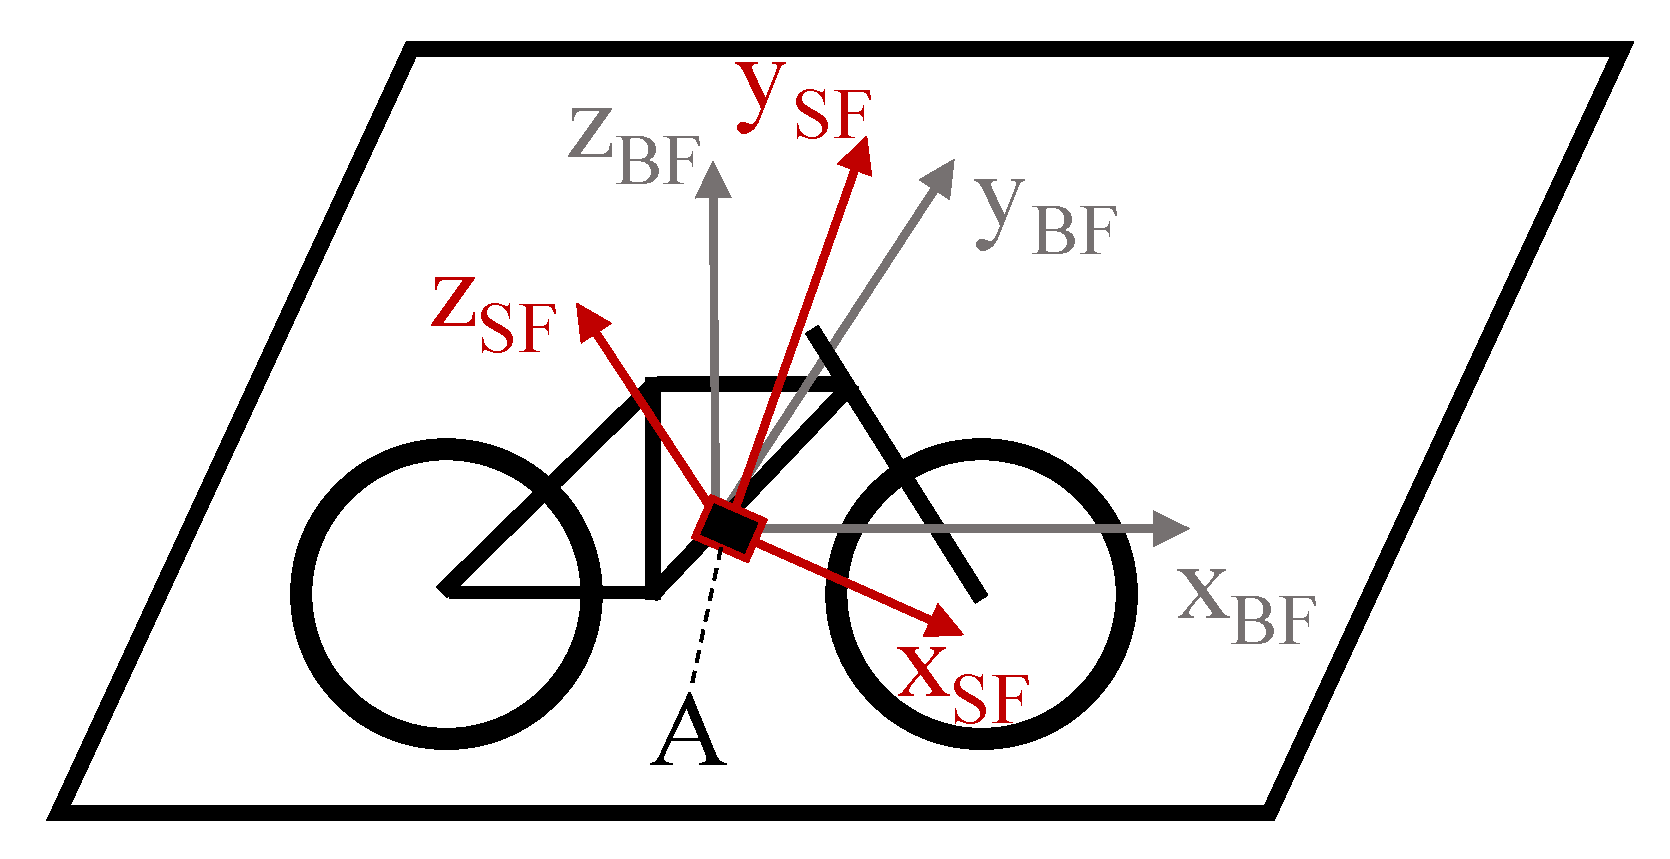
\includegraphics[width=0.7\linewidth]{Bilder/AchsenSensor_Bike.png}
	\caption{Achsenrichtung in Sensorframe sowie in Bikeframe \citep{SchneeCorrection2020}}
	\label{fig:AchsenSensor_Bike}
\end{figure}



\subsection{Übersicht der bereits erkennbaren Unfälle}

%- Erkannte Szenarien/Fälle\\
%
%- Zusammengefasste Tabelle von Jan (Vollständige Tabelle im Anhang)

In der \autoref{fig:Entscheidungsbaum_Jan} ist der Entscheidungsbaum abgebildet, wonach eine Unfallklassifizierung erfolgt wird. Die Einzelkomponenten (CollisionHit, GroundHit, TipOver) werden später separat erläutert.
\begin{figure}[H] % TODO: Eine Tabelle mit der ID-erklrung hinzufügen und darauf beziehen
	\centering
	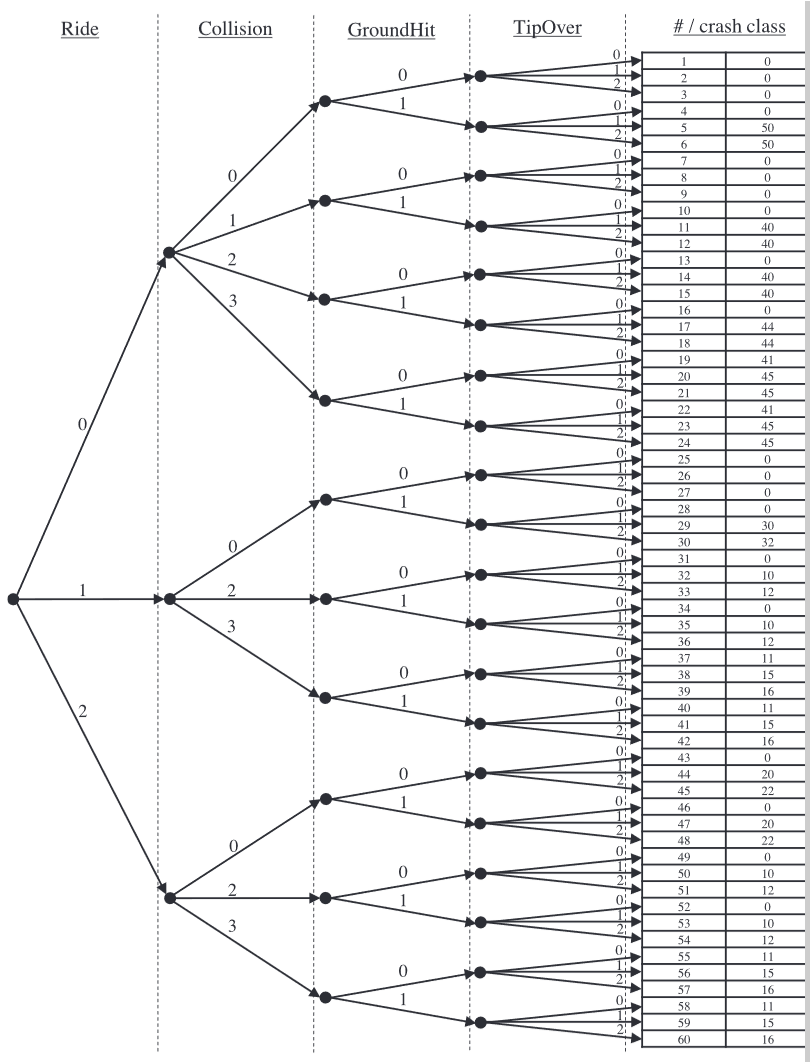
\includegraphics[width=\linewidth]{Bilder/Entscheidungsbaum_Jan.png}
	\caption{Entscheidungsbaum des Unfallerkennungsalgorithmus'\citep{Schneeclassification2021}}
	\label{fig:Entscheidungsbaum_Jan}
\end{figure}

\begin{figure}[H] %TODO: darauf eingehen.
	\centering
	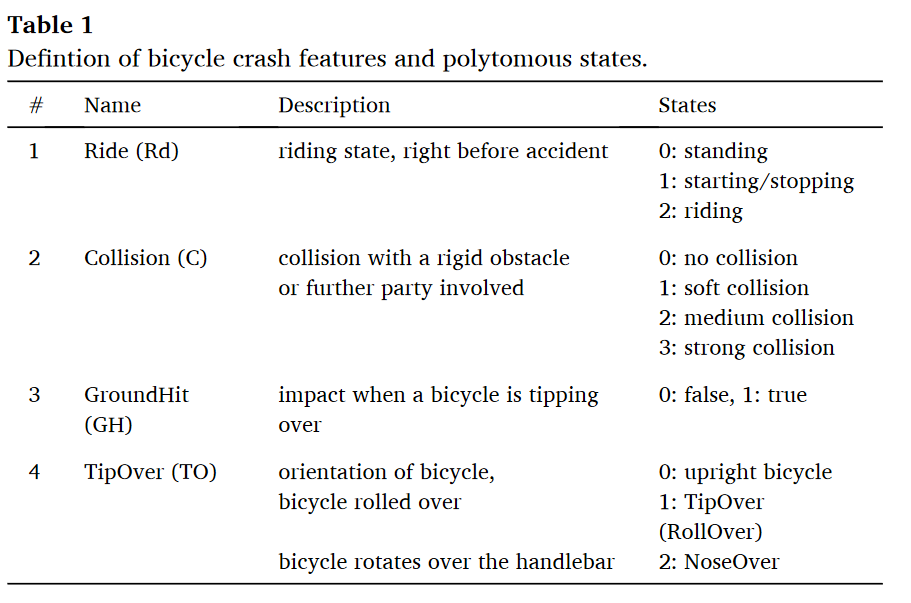
\includegraphics[width=0.6\linewidth]{Bilder/AlgoTabaIDs.png}
	\caption{Definition der IDs aus der \autoref{fig:Entscheidungsbaum_Jan}\citep{Schneeclassification2021}}
	\label{fig:AlgoTabaIDs}
\end{figure}


%\subsection{Einzelkomponenten des Unfallerkennungsalgorithmus'}
\subsection{1. Komponente: TipOver}
%
%
%
%
Diese Komponente kontrolliert den Neigungswinkel des Motorrads und stellt fest, wenn das Motorrad umkippt.

Bei Motorradunfällen auf Straßen, die sich im Anschluss an eine Kurve ereignen, stellt sich immer wieder die Frage nach der maximalen Geschwindigkeit, mit der die Kurve auf einem Motorrad durchfahren werden konnte.
Um das Motorrad durch die Kurve zu bewegen, muss sich der Fahrer mit seiner Maschine in die Kurve legen. Während einer Fahrt in der Kurve wirken zwei Kräfte $(F_q)$ und $(F_G)$ am Motorrad (\autoref{fig:VereinfachteDarstellungDerKraefteBeiStationaererKurvenfahrt}).

Wenn der Kraft $(F_q)$ größer als $(F_G)$ tritt, kippt das Motorrad um. Im normalen Fall soll
\begin{align*}
	F_G \geq F_q
\end{align*}
immer gültig sein.

D.h. 
\begin{align*}
	\frac{F_q}{F_G} \leq 1
\end{align*}
Beim Einsetzen in der \autoref{gl:Schraegwinkel} ergibt sich der maximale zulässige Winkelwert:

\begin{align*} \lambda_{zul} \leq \arctan(1) \leq \ang{45}\end{align*}

D.h. Bei einer Neigung von über $\ang{45}$, sollte das Motorrad umkippen. Sollte der Fahrer das Fahrstil '''Hängen''' verwenden, könnte er eine größere Neigung erfolgen, ohne zu rutschen.

Das Modell "'TipOver"' erkennt den Fall, in dem der Winkel über den Schwellwert liegt, und gibt dem Entscheidungsmodell eine Meldung weiter.



\subsection{2. Komponente: GroundHit}
%
%
%
%

Dieses Modell dient dazu, den Schlag zu erkennen, wenn das Motorrad am Boden ankommt. Dieses Modell geht von der Energie aus der \autoref{gl:EnergieFormel_JanPaper} aus. Es hat einige Spezifikationen, die die verschiedene Szenarien abdeckt. Zwei typische Szenarien sind in der \autoref{fig:BicycleGroundHit2Angles} dargestellt. Die \autoref{fig:BicycleGroundHit2Angles1} zeigt der Fall, wenn ein Fahrrad nach einer ursprünglichen aufrechten Position umkippt, und die \autoref{fig:BicycleGroundHit2Angles2} das Umkippen eines Fahrrads mit einer ursprünglichen Neigung (z.B. in einer Kurve).
Die Energie vom GroundHit im zweiten Fall ist deutlich kleiner, deswegen wird der Schwellwert nach dem Neigungswinkel angepasst. Je größer die Motorradneigung ist, desto kleiner ist der GroundHit-Schwellwert.\\

\begin{figure}[H]
	\centering
	\begin{subfigure}{0.49\textwidth}
		\centering
		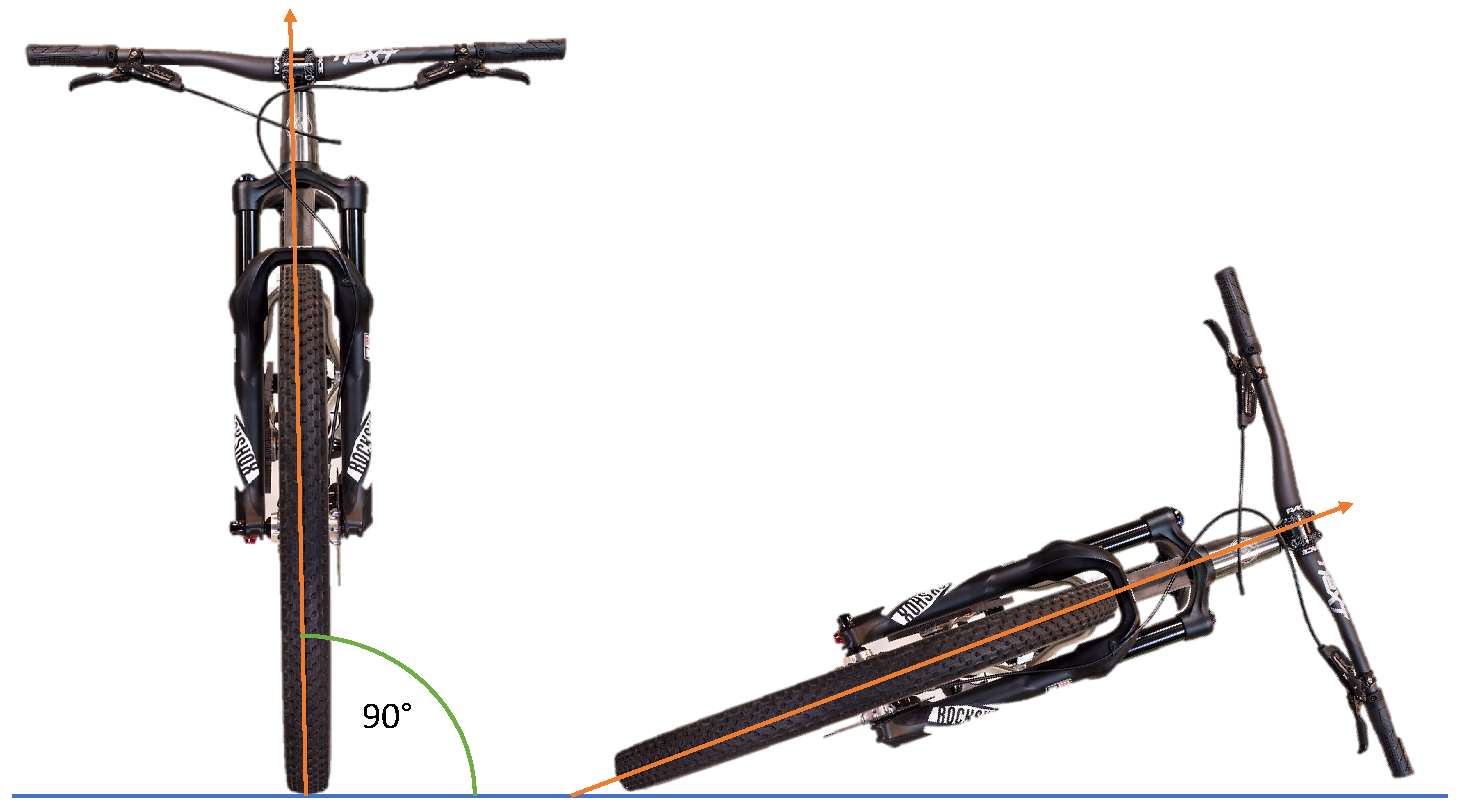
\includegraphics[page = 1, width=\textwidth]{Bilder/BicycleGroundHit2Angles.pdf}
		\caption{Beispiel eines aufrechten Fahrrads beim Umkippen}
		\label{fig:BicycleGroundHit2Angles1}
	\end{subfigure}
%	\hfill
	\begin{subfigure}{0.49\textwidth}
		\centering
		\includegraphics[page = 2, width=\textwidth]{Bilder/BicycleGroundHit2Angles.pdf}
		\caption{Beispiel eines Fahrrads mit einer Neigung beim Umkippen}
		\label{fig:BicycleGroundHit2Angles2}
	\end{subfigure}
	\caption{Beispiel eines Fahrrads beim Umkippen mit einer ursprünglichen aufrechten Postion sowie Neigung}
	\label{fig:BicycleGroundHit2Angles}
\end{figure}

Nachdem das Modell den Bodenschlag erkennt, wird eine Meldung dem Entscheidungsmodell weitergegeben. Demnächst werden zwei Beispiele zum besseren Verständnis erläutert.

\subsubsection{Beispiele 1: Kein GroundHit}
In diesem Beispiel ist eine Testfahrt ohne GroundHit durchgeführt und schließlich analysiert. Nach der Fahrt und bei späterer Simulation wurde entdeckt, dass die Kalibrierung nicht richtig war und musste manuell in der Simulation angepasst werden. Eine Rotationsmatrix, die in der Regel durch die Kalibrierung gerechnet und umgesetzt wird, wurde hier manuell erstellt und verwendet. Um eine falsche Nachkalibrierung zu verhindern, wurde der zuständige Teil deaktiviert. Es ist wichtig zu wissen, dass die Position des Geräts sich während der Fahrt kaum verändert hat.

%\begin{figure}[H]
%	\centering
%	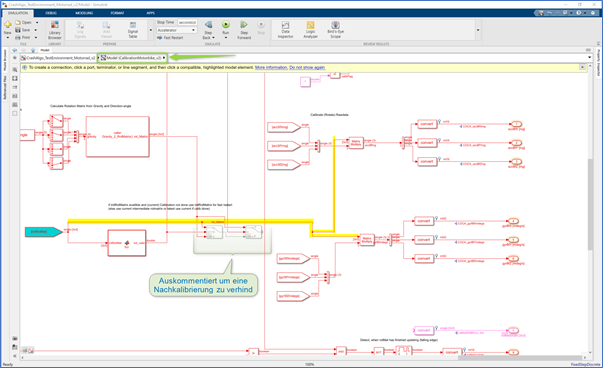
\includegraphics[width=\linewidth]{Bilder/KalibModul_Nachkaklib_deaktiviert.png}
%	\caption{Darstellung einer deaktivierten Nachkaklibrierung}
%	\label{fig:KalibModul_Nachkaklib_deaktiviert}
%\end{figure}


In der \autoref{fig:GH_Testfahrt_noGroundHit_EnergyZoomed} ist der Fall vorgestellt, in dem kein Groundhit erkannt wurde. Während dieser Fahrt fand ebenfalls kein Unfall statt. 
Die oberen Grafiken zeigen die Geschwindigkeit (blau) sowie die GroundHit-Auslösungen, die entweder im Feld (grün) oder durch die Simulation (orange) gefeuert wurde, über die Zeit.
Die unteren Grafiken stellen die kinetische Energie (blau) aus der \autoref{gl:EnergieFormel_JanPaper} sowie den Energieschwellwert (orange) über die Zeit dar.
Die zwei rechte Grafiken veranschaulichen einen kleinen kritischen Bereich der jeweiligen Signalen, damit der Signalverlauf an der Stelle klar betrachtet wird.
%Es wurde allerdings mehrere Szenarien getestet, die im Pocket-Mode vorkommen können. Z.B. laufen mit einer aktivierten Unfallerkennung oder beim Fahren an der Ampel bremsen und den Fuß auf dem Boden runterstellen mit dem Smartphone in der Hosentasche.

%\begin{figure}[H]
%	\centering
%	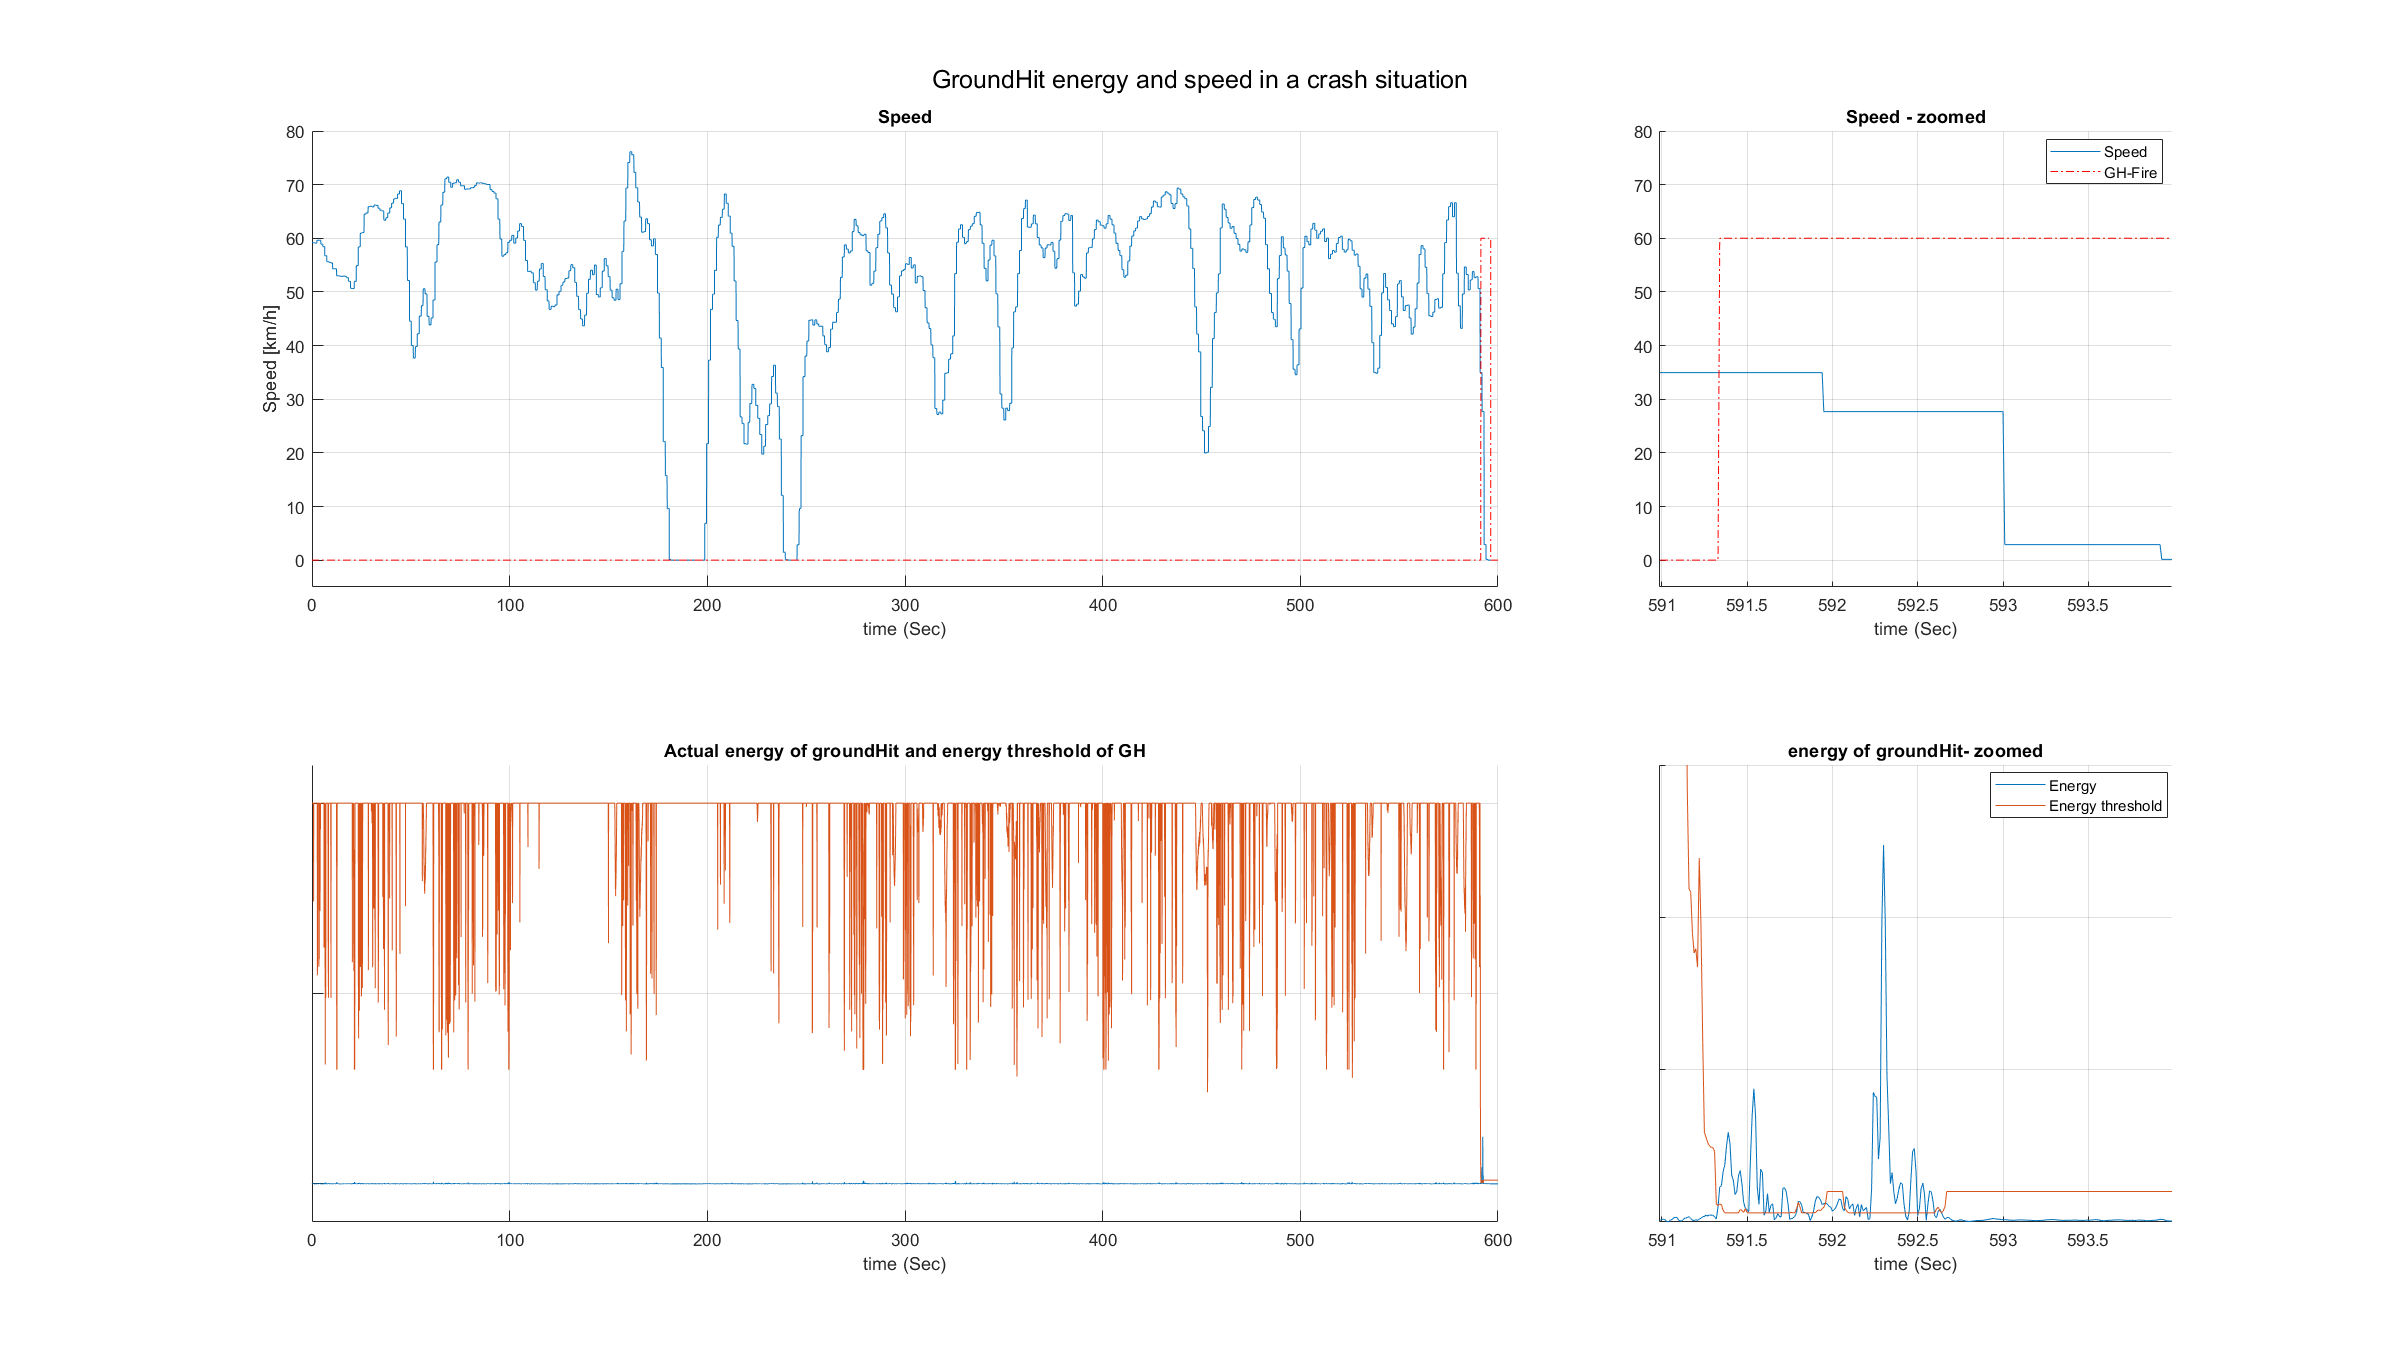
\includegraphics[width=\linewidth]{Bilder/GH1_speed_GHEnergy.png}
%	\caption{Testfahrt ohne GroundHit}
%	\label{fig:GH_Testfahrt_noGroundHit_FullView}
%\end{figure}
\begin{figure}[H] %TODO: richtige Fall zeigen (erste Testfahrt von Nino)
	\centering
	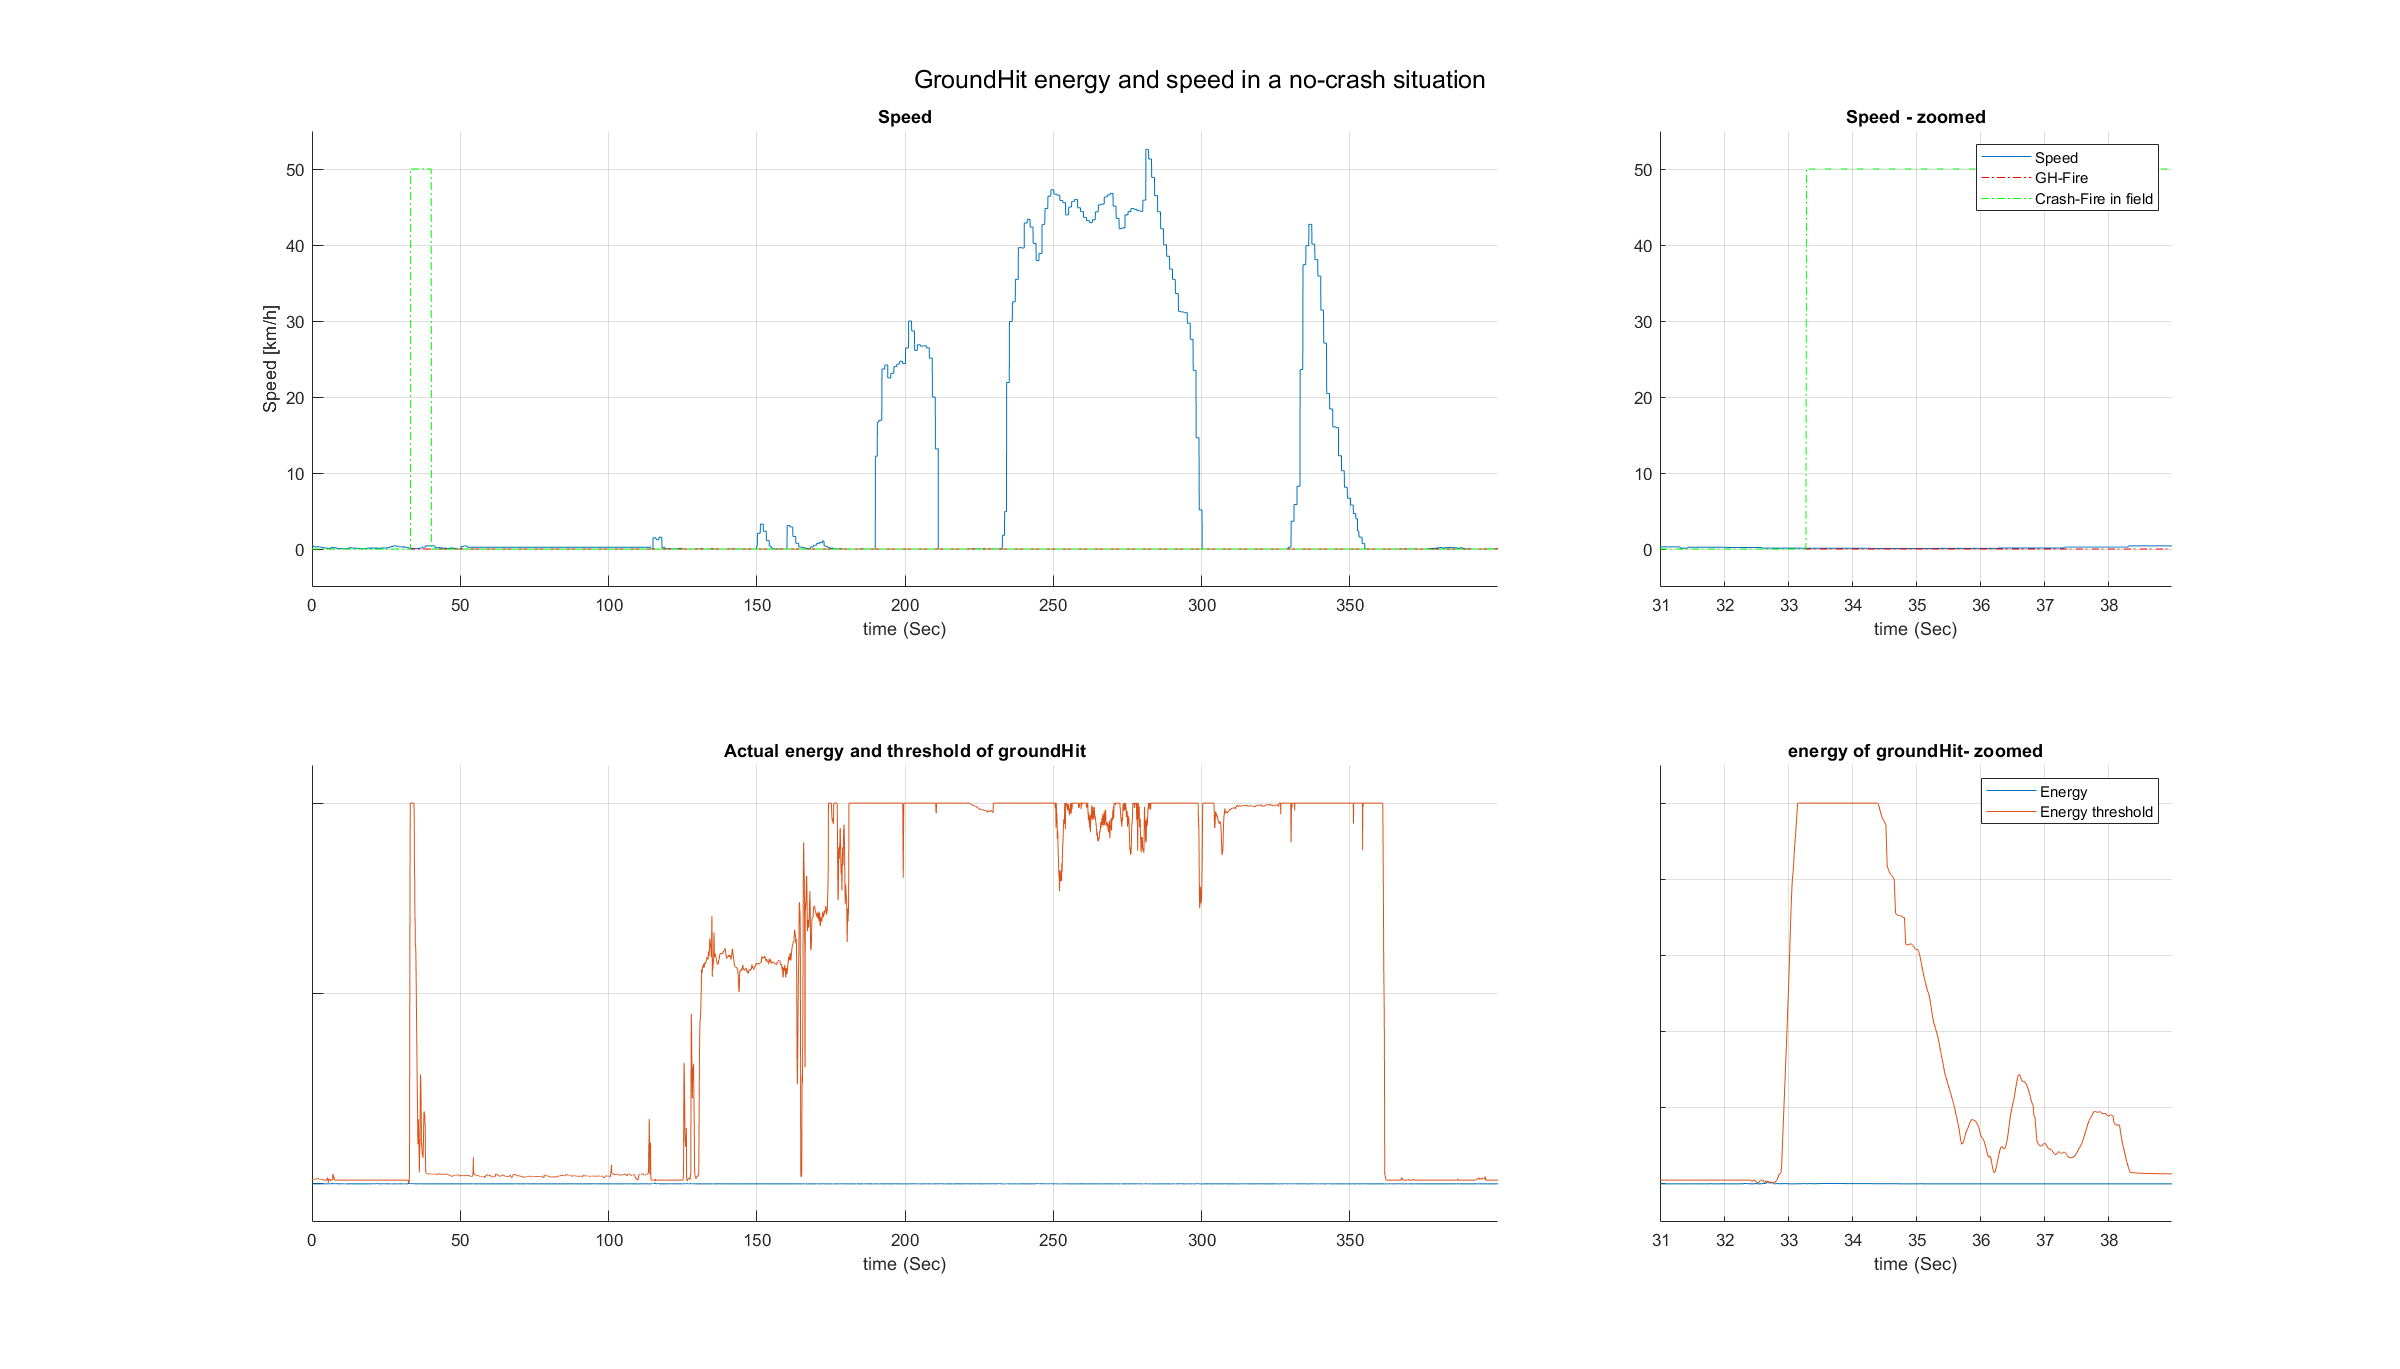
\includegraphics[width=\linewidth]{Bilder/GH3_speed_GHEnergy_TestFahrt.png}
	\caption{Verlauf der Energie sowie des Energieschwellwerts bei einer Testfahrt ohne GroundHit}
	\label{fig:GH_Testfahrt_noGroundHit_EnergyZoomed}
\end{figure}
%In der \autoref{fig:GH_Testfahrt_noGroundHit_EnergyZoomed} ist zum Zeitpunkt 32,7 s Folgendes abzulesen:
%\begin{itemize}
%	\item $RideFire = 0$, keine Fahrt
%	\item $accEnergyStXYintern = 0,007$
%	\item $GH_ScalexGHEnergythreshold = 0,004$
%	\item $TO_curAngle_deg = 12$
%	\item $eulerPitch_deg$ springt von ca. -60 auf ca. +60 (Das handy wurde wahrscheinlich um 180 gedreht. Das könnte auch durch die Acc-Daten bestätigt werden)
%\end{itemize}

An dieser Stelle hat die tatsächliche Energie (blau) den Schwellwert (orange) nicht überschritten, was eigentlich keinen GroundHit-Alarm auslösen soll. Während der Fahrt hat das Smartphone an der Stelle einen falschen Alarm ausgelöst, da die Kalibrierung nicht $100\%$ richtig war. In den simulierten Daten wurde diese angepasst und hat dazu geführt, keinen Unfall zu erkennen.

\subsubsection{Beispiele 2: Unfall mit GroundHit}
In der \autoref{fig:RealcrashID_2806_EnergyZoomed_MitGroundHit} sind die simulierten Daten einer echten Fahrt mit einem Unfall dargestellt. 
%Es ist zu bemerken, dass die $GH_SaleXGHEnergythreshold$ von dem Winkel ($tipOverAngle_deg$) abhängig ist. Bei einem hohen Winkel sinkt die $SaleXGHEnergythreshold$ (die linke unterste Darstellung der \autoref{fig:RealcrashID_2806_FullView_MitGroundHit}).

%\begin{figure}[H]
%	\centering
%	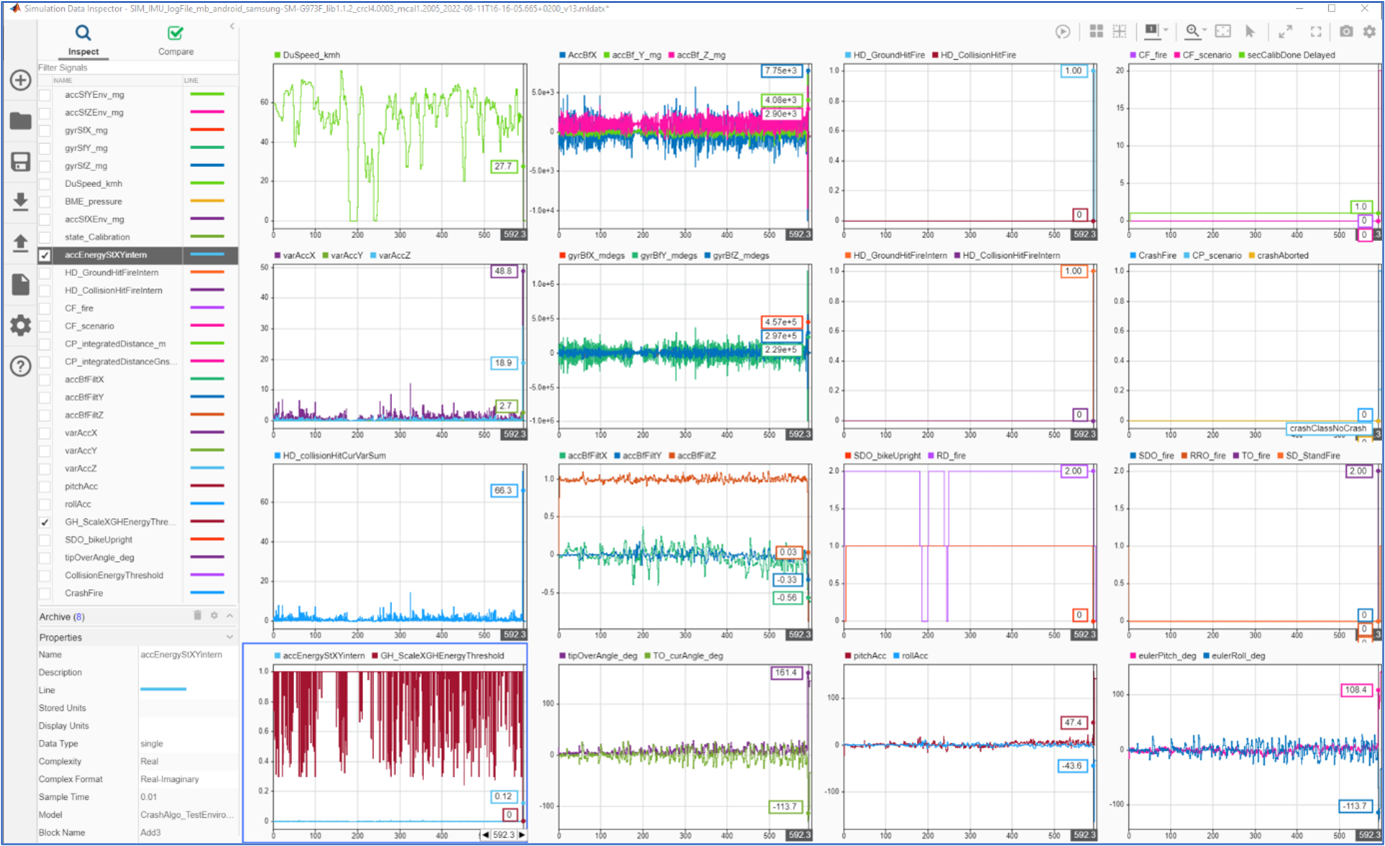
\includegraphics[width=\linewidth]{Bilder/RealcrashID_2806_FullView_MitGroundHit.png}
%	\caption{Crash mit GroundHit - ID 2806 - Full View}
%	\label{fig:RealcrashID_2806_FullView_MitGroundHit}
%\end{figure}
\begin{figure}[H]
	\centering
	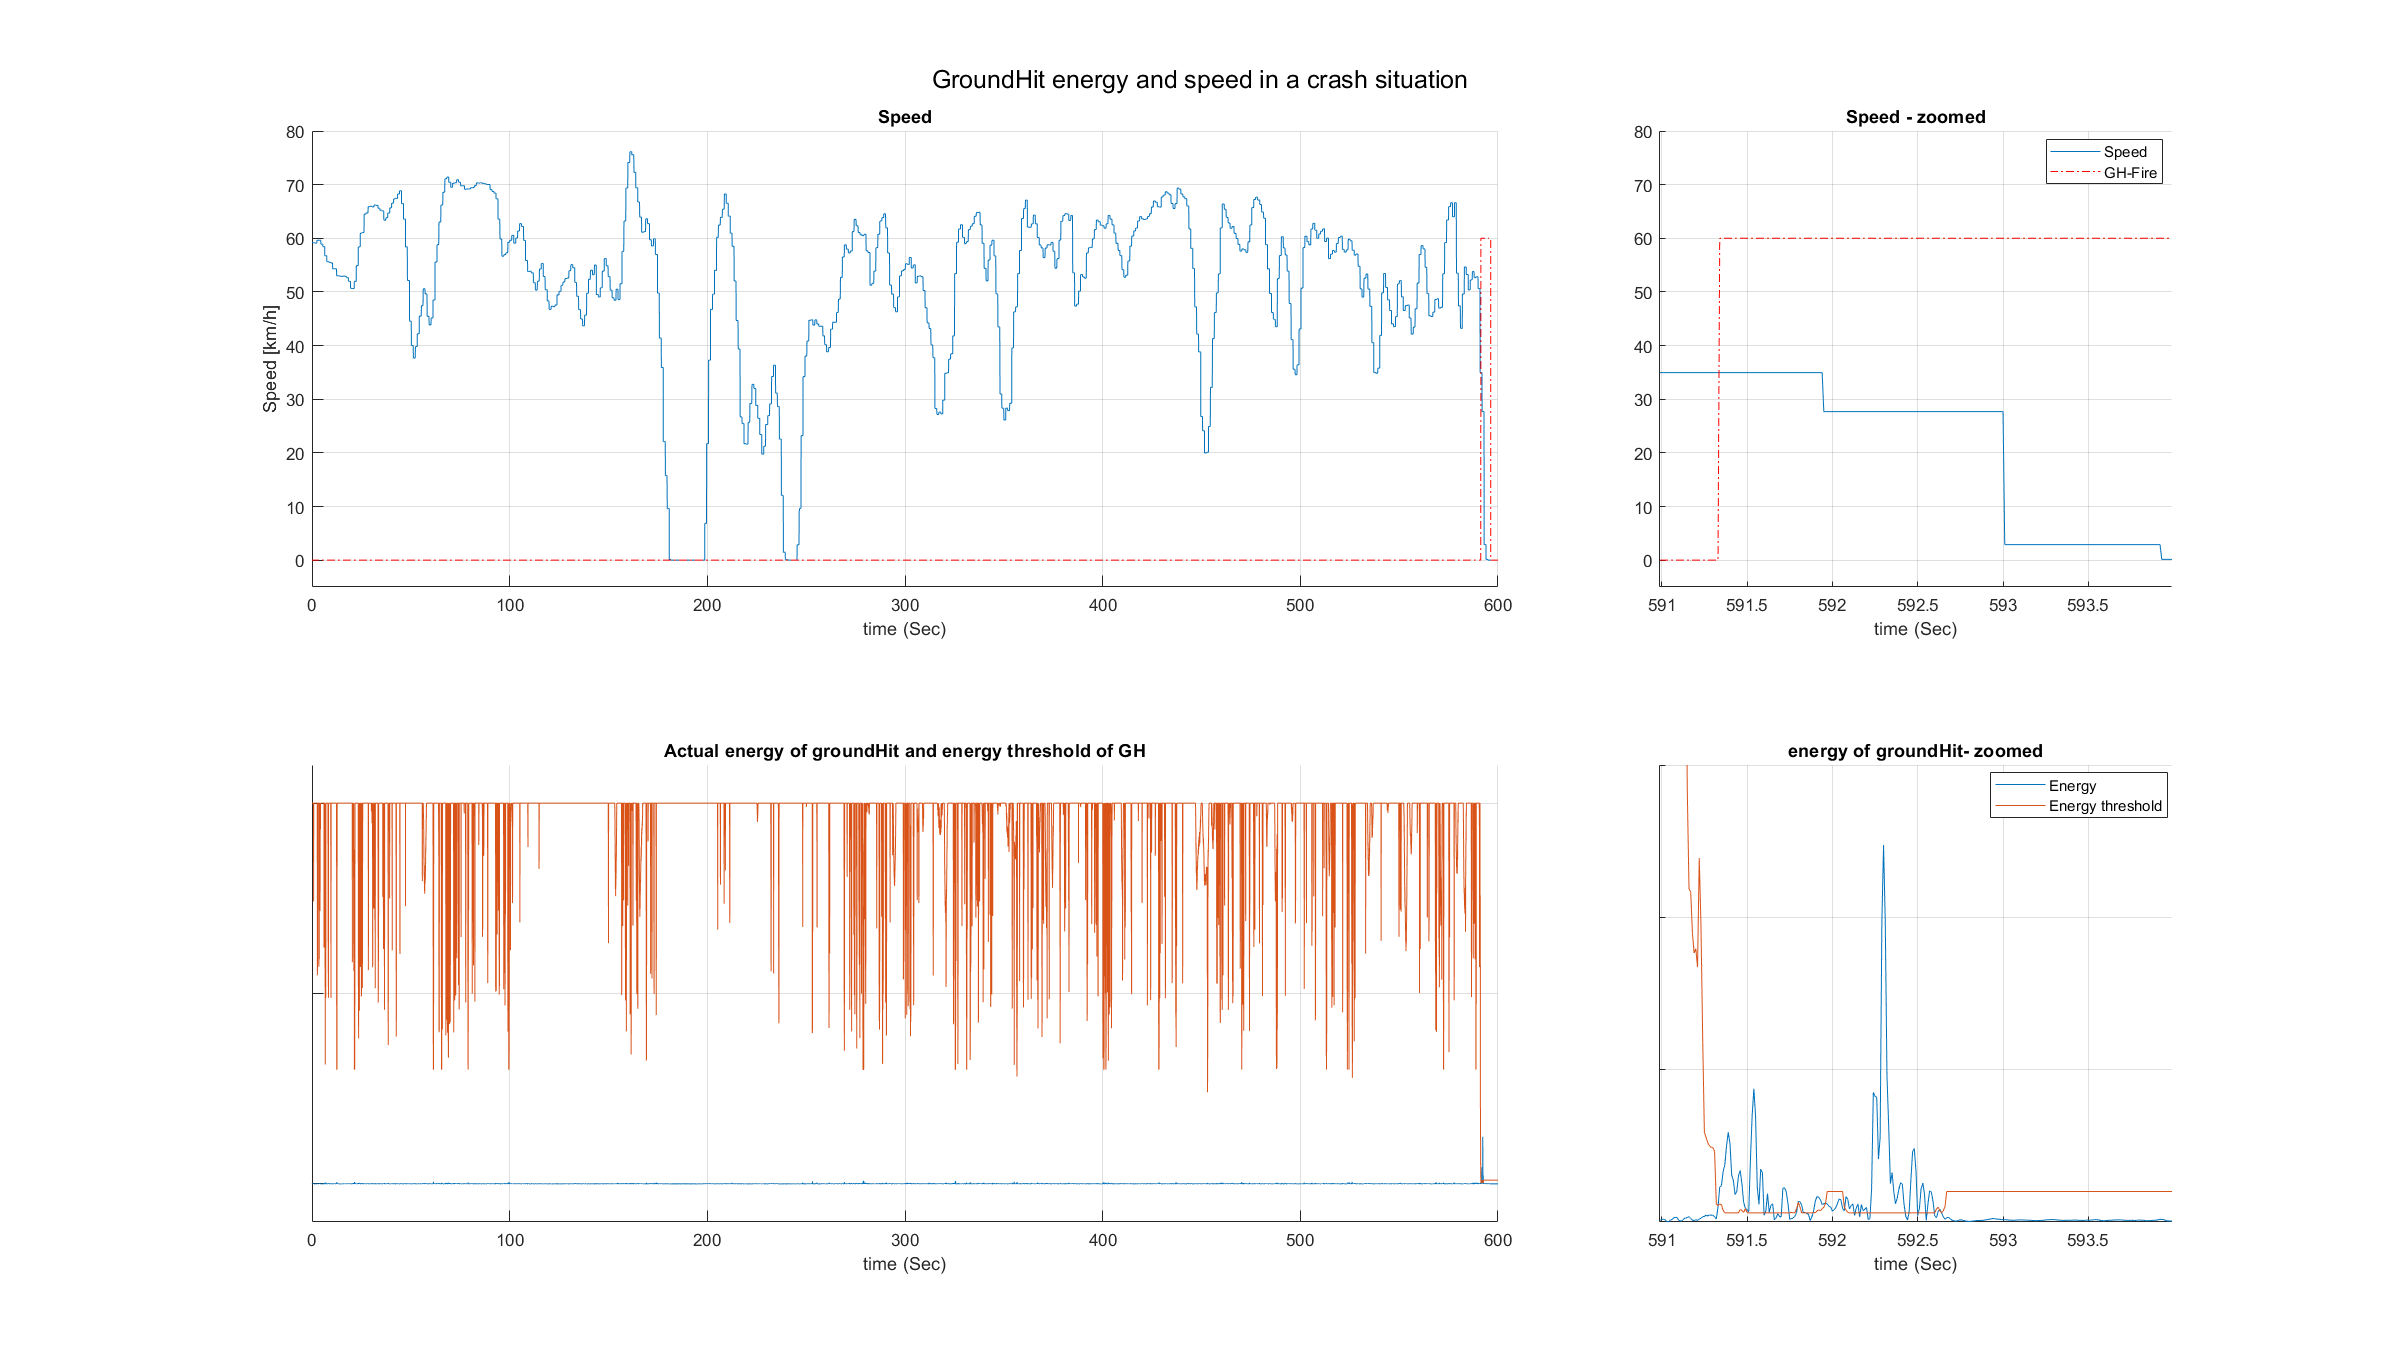
\includegraphics[width=\linewidth]{Bilder/GH1_speed_GHEnergy.png}
	\caption{Verlauf der Energie sowie des Energieschwellwerts bei einer Echtfahrt mit GroundHit} %  ID 2806
	\label{fig:RealcrashID_2806_EnergyZoomed_MitGroundHit}
\end{figure}
In der \autoref{fig:RealcrashID_2806_EnergyZoomed_MitGroundHit} sind die Daten eines Unfalls dargestellt und auf die Unfallphase gezoomt. 
Die oberen Grafiken stellen die Geschwindigkeit (blau) sowie die GroundHit-Auslösung (orange) über die Zeit dar.
Die unteren Grafiken zeigen die kinetische Energie (blau) aus der \autoref{gl:EnergieFormel_JanPaper} sowie den Energieschwellwert (orange) im Laufe der Zeit.
Die zwei rechte Grafiken veranschaulichen einen kleinen Bereich der jeweiligen Signalen, in dem einen Unfall aufgetreten ist.

In der Abbildung ist zu erkennen, dass der Energieschwellwert bei der Sekunde 591 stark sinkt, da an der Stelle der Neigungswinkel ebenfalls größer wird.
An dieser Stelle wird diesen Wert von der tatsächlichen kinetischen Energie überschritten, was eine Alarmauslösung feuern muss. Die obere rechte Grafik zeigt die Auslösung an der gleichen Stelle, an der den Schwellwert überschritten wird.

%wo die $accEnergyStXYintern > GH_SaleXGHEnergythreshold$ ist (ca. 591,35 s), ist der Winkel fast gleich 45 -> dadurch löst ein Alarm der GroundHit aus. Das entspricht die Erwartungen.


%\subsubsection{Beispiele 3: Unfall mit GroundHit}


\subsection{3. Komponente: CollisionHit} %TODO: Abschnitt erweitern und ebenfalls umformulieren
%Beispiel...
%\begin{table}
%	\centering
%	\caption{Entscheidungsschema eines statistischen Tests}
%	\begin{tabular}{l| l r}%p{2.8cm}|>{\centering\arraybackslash}p{4.5cm}>{\centering\arraybackslash}p{4.5cm}}
%		\toprule %\hline
%		& \multicolumn{2}{S}{\textbf{Ist \boldsymbol{$H_0$} tatsächlich wahr?}}\\
%%		\cline{2-3}
%		\textbf{Test} & \textbf{Ja} & \textbf{Nein}\\
%		\midrule
%		\textbf{verwirft \boldsymbol{$H_0$}} & {Fehler 1. Art ($\alpha$)} & richtige Entscheidung\\
%%		\hline
%		\textbf{nimmt \boldsymbol{$H_0$} an} & richtige Entscheidung & {Fehler 2. Art ($\beta$)} \\
%		\bottomrule %\hline
%	\end{tabular}
%\label{tab:EntscheidungsschemaStatistischenTests}
%\end{table}
P.S: EnergyThreshold ändert sich nach Geschwindigkeit und Rollwinkel (Ab \ang{45}).\\

\begin{figure}[H] %TODO: ein fall aus der atenbank vorstellen!
	\centering
	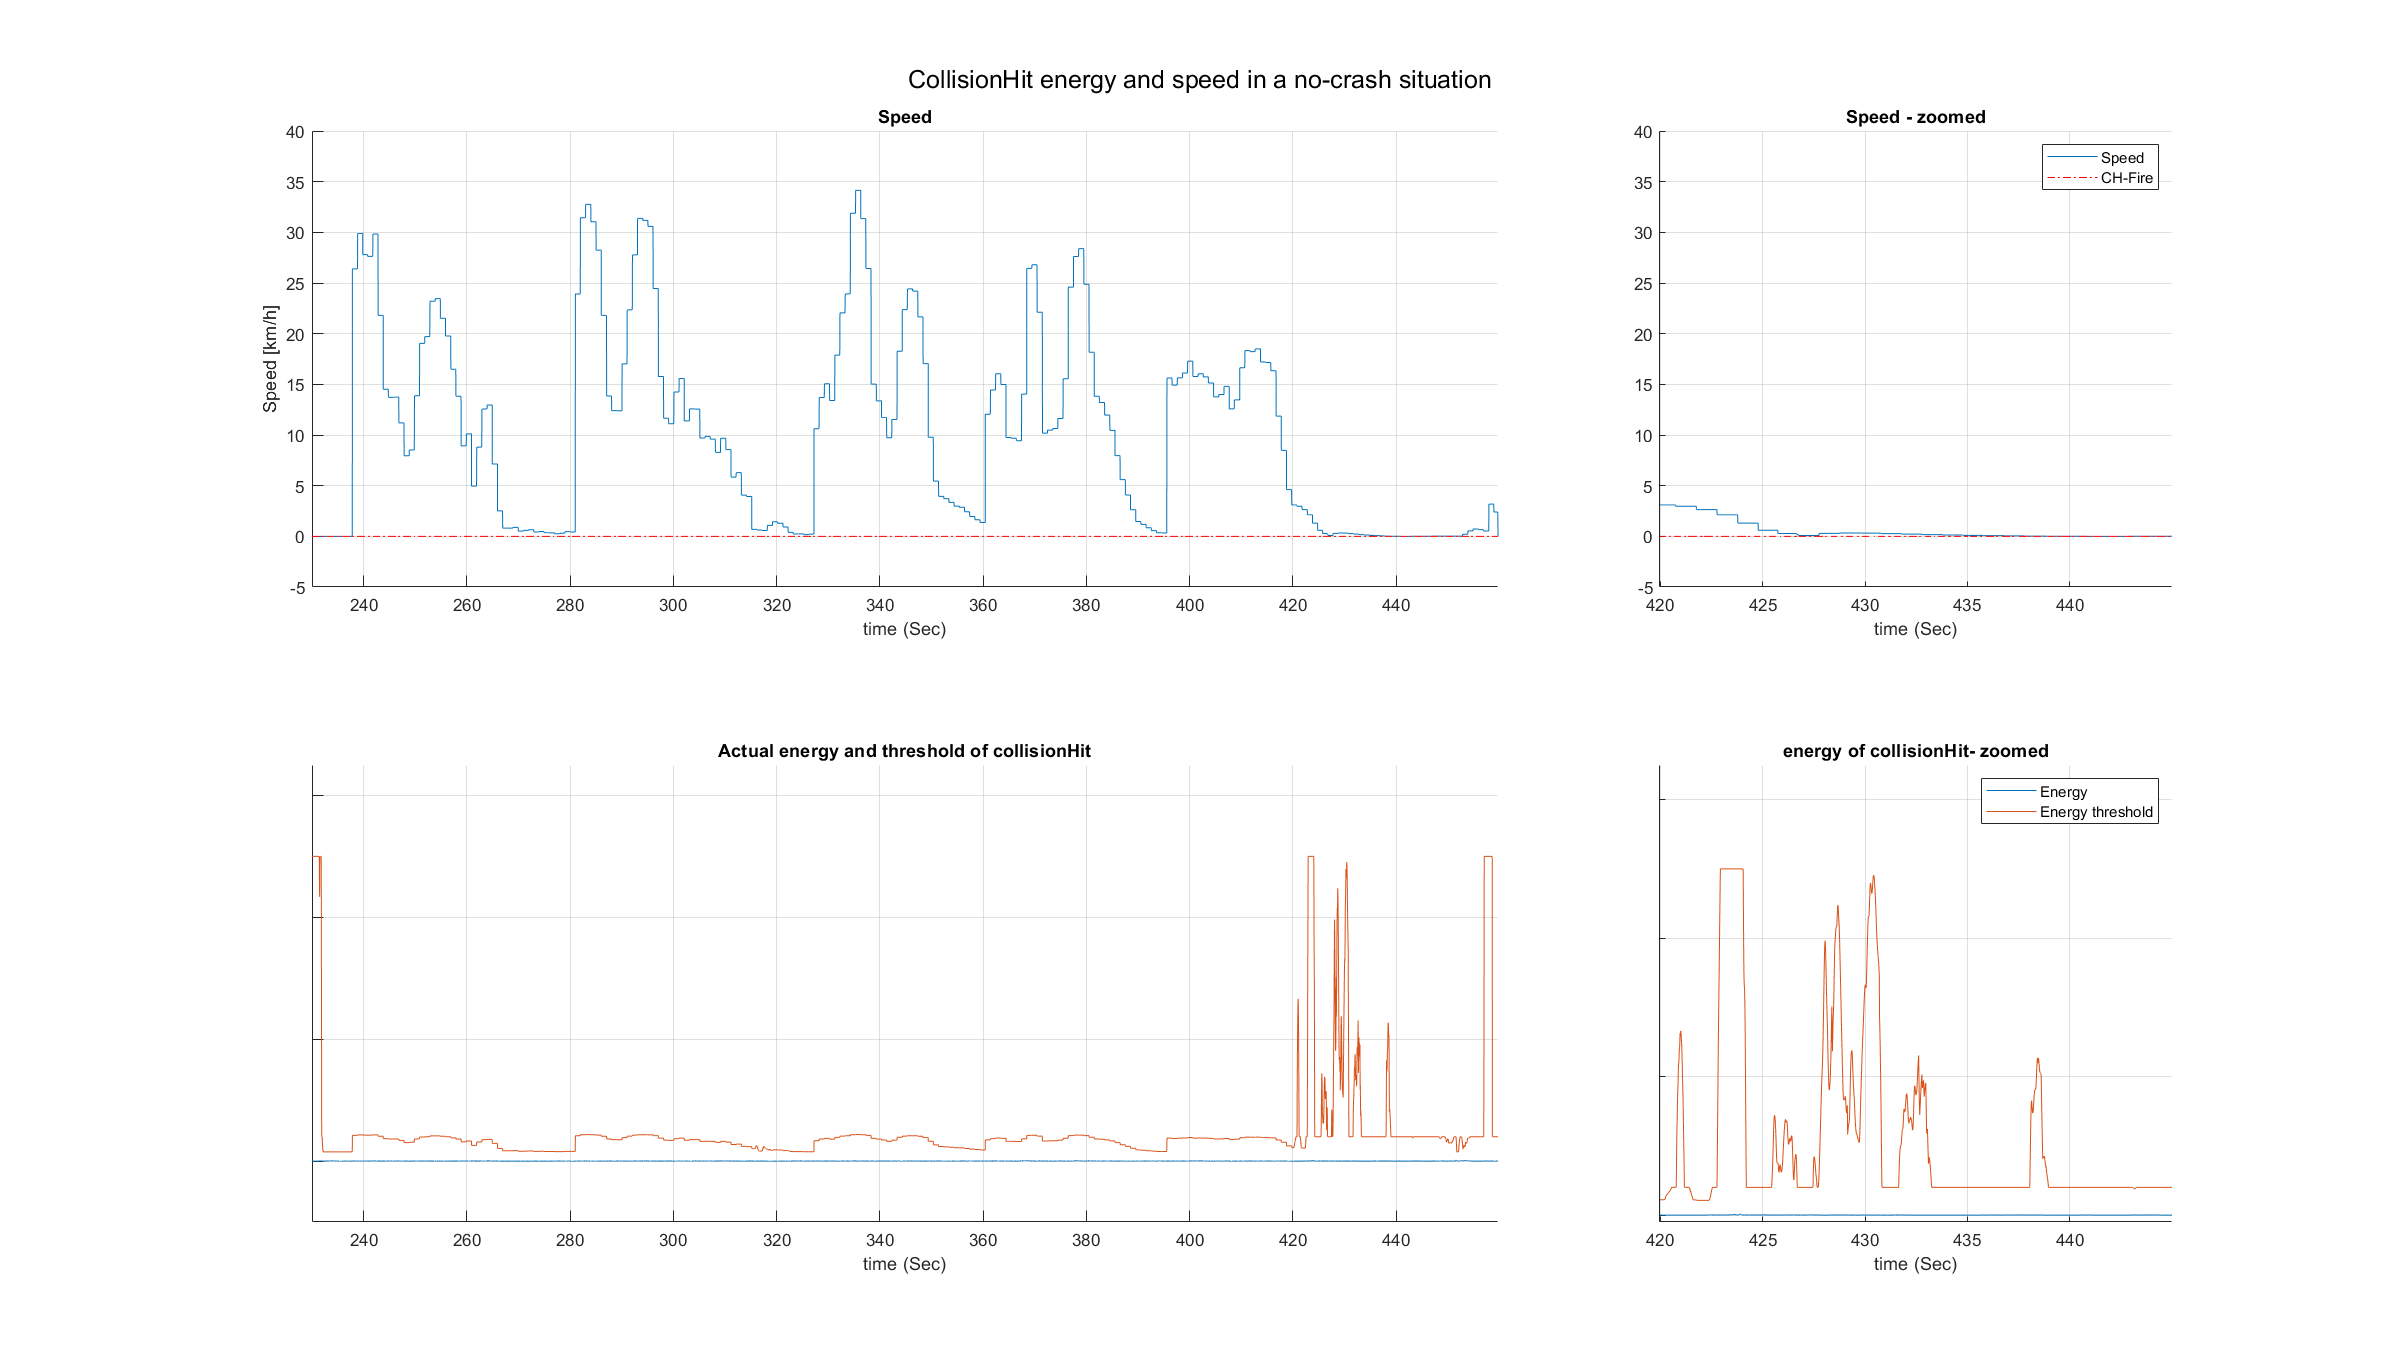
\includegraphics[width=\linewidth]{Bilder/CH1_speed_CHEnergy.png} % ID: 2546
	\caption{Verlauf der Energie sowie des Energieschwellwerts bei einer Echtfahrt ohne CollisionHit}
	\label{fig:CH_ID_2546_FullView}
\end{figure}

In der \autoref{fig:CH_ID_2546_FullView} ist der Fall vorgestellt, in dem keine Kollision erkannt wurde. Während dieser Fahrt fand ebenfalls kein Unfall statt. 
Die oberen Grafiken zeigen die Geschwindigkeit (blau) sowie die CollisionHit-Auslösung (orange) über die Zeit.
Die unteren Grafiken stellen die kinetische Energie (blau) sowie den Energieschwellwert (orange) über die Zeit dar.
Die zwei rechte Grafiken veranschaulichen einen kleinen Bereich der jeweiligen Signalen, wo eine Überschneidung der Signalen nicht klar ist.

Aus der Grafiken ist zu bemerken, dass der Schwellwert der Energie nicht überschritten wird, auch wenn der stark sinkt. Das entspricht ebenfalls den Erwartungen.

\begin{figure}[H]
	\centering
	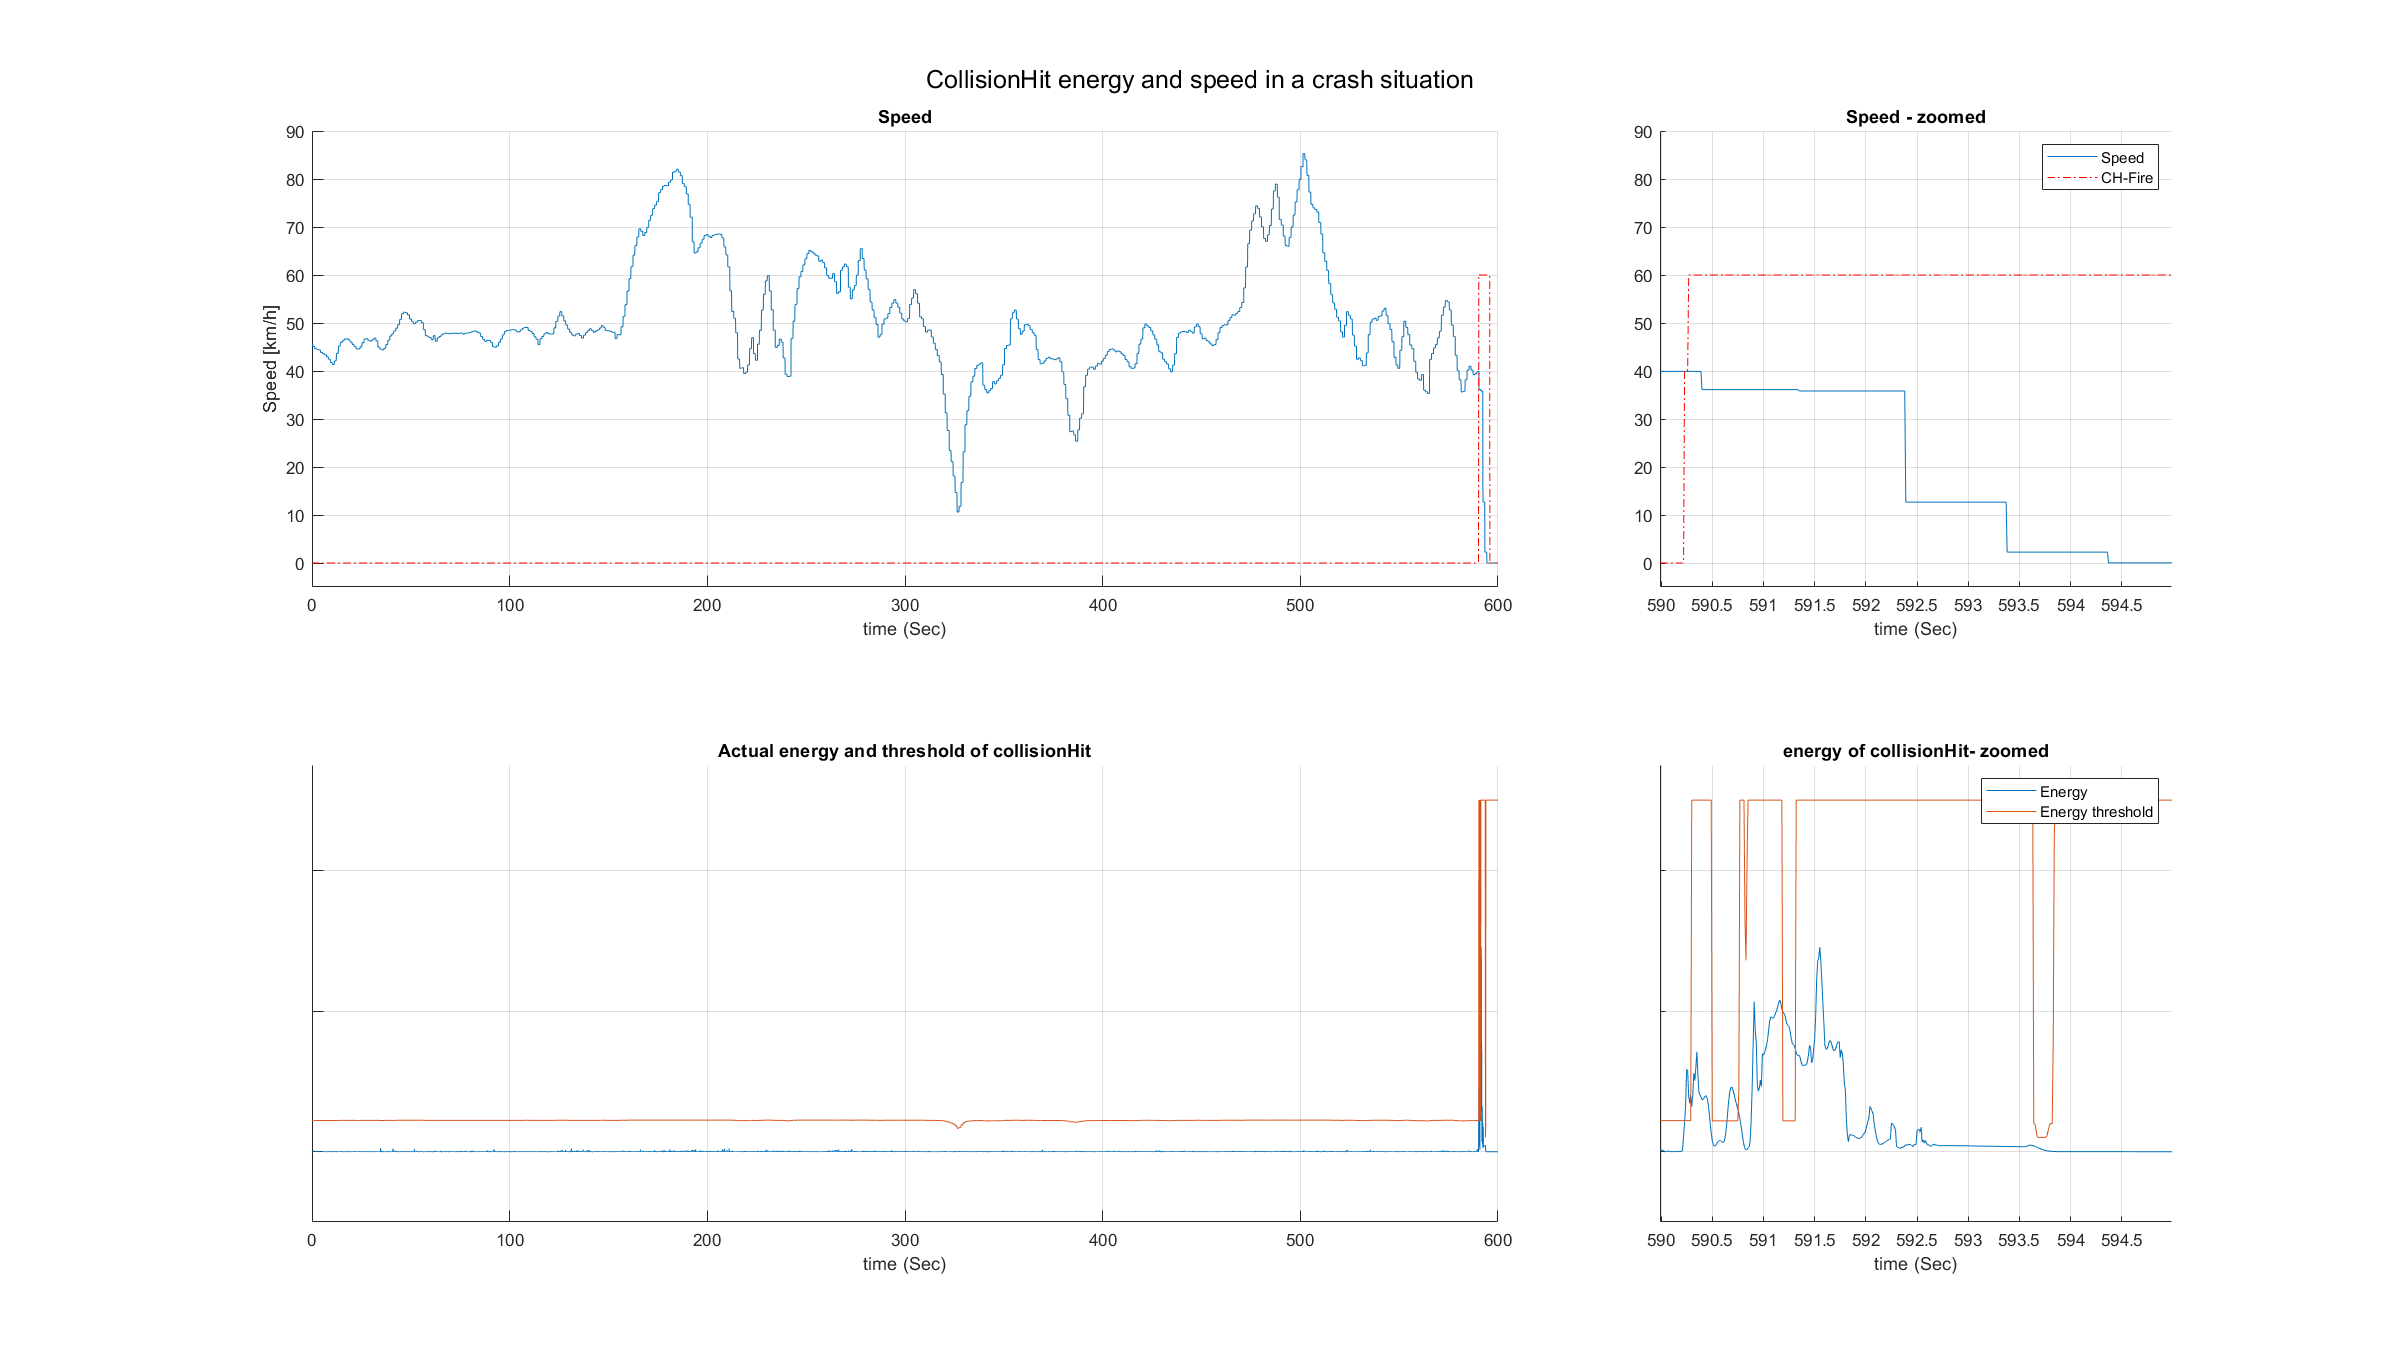
\includegraphics[width=\linewidth]{Bilder/CH2_speed_CHEnergy.png}
	\caption{Verlauf der Energie sowie des Energieschwellwerts bei einer Echtfahrt ohne CollisionHit} % ID 2546
	\label{fig:CH_ID_2546_zoom}
\end{figure}

Analog dazu ist in der \autoref{fig:CH_ID_2546_zoom} der Fall vorgestellt, in dem eine Kollision erkannt wurde. Während dieser Fahrt fand ebenfalls auch ein Unfall statt. 
Die oberen Grafiken zeigen die Geschwindigkeit (blau) sowie die CollisionHit-Auslösung (orange) über die Zeit.
Die unteren Grafiken stellen die kinetische Energie (blau) sowie den Energieschwellwert (orange) über die Zeit dar.
Die zwei rechte Grafiken veranschaulichen einen kleinen Bereich der jeweiligen Signalen, wo eine Überschneidung der Signalen nicht klar ist.




